Los estudios sobre el estado del conductor son cada vez más frecuentes, ya que además de mejorar la experiencia de la conducción, supone un incremento en la seguridad del vehículo. La presencia de sistemas de asistencia ha permitido expandir el conocimiento en este campo, ya que a través de esta información se pueden hallar soluciones a ciertas necesidades del conductor mediante estímulos tanto auditivos como visuales. El desarrollo de estas tecnologías pretende avanzar hacia la integración total de los vehículos autónomos en el tráfico mixto, al igual que la implementación de algoritmos de toma de decisiones más sofisticados y realistas. 

Sin embargo, todavía existen situaciones confusas donde el vehículo requiere la intervención del conductor para resolverlas. Este hecho sugiere una falta de reglas de decisión ya que, a pesar del conocimiento adquirido por los sensores, el sistema carece de recursos que el conductor sí posee de manera natural.

La acción de conducir se basa principalmente en la percepción del entorno, siendo los sensores en los vehículos autónomos los homólogos al sistema visual humano. La principal fuente de información de un conductor humano son los ojos, la cual precede a los procesos cognitivos que definen la toma de decisiones y las acciones posteriores. Los sistemas de seguimiento visual o eye-tracking, son comúnmente utilizados para el análisis del comportamiento visual del conductor, donde se pueden extraer conclusiones sobre su estado y su atención (\cite{werneke}; \cite{lemonnier}; \cite{vetturi}). Variables atencionales como el diámetro de la pupila, la posición de la mirada en el espacio, las sacadas y las fijaciones, son ampliamente estudiadas por la comunidad científica. 

Con todo lo anterior, en este capítulo se evalúa el comportamiento visual del conductor en diferentes escenarios complejos, con objeto de observar si las variables atencionales se ven afectadas. Los principales escenarios analizados en vías de alta capacidad son:

\begin{enumerate}
    \item \hyperref[31]{Incorporaciones a una vía principal en conducción manual} 
    \item \hyperref[32]{Adelantamientos en conducción parcialmente automatizada} 
\end{enumerate}

La elección de estas situaciones es debido a la alta velocidad de respuesta requerida por el entorno y los numerosos parámetros a valorar de manera simultánea en la toma de decisiones. Los resultados que se obtengan aportarán información sobre cómo un conductor gestiona situaciones complejas y de qué manera un vehículo autónomo podría abordarlas de manera similar.

\section{Incorporación a una vía principal en conducción manual}\label{31}

La maniobra de incorporación se considera uno de los entornos más complejos de la conducción en autovías y autopistas. En esta situación, la carga cognitiva del conductor se ve acrecentada por una gran cantidad de información a procesar simultáneamente, como la velocidad óptima de incorporación, distancia a los vehículos adyacentes y el hueco disponible. Este entorno puede ser además conflictivo en presencia de un mayor volumen de tráfico, debiendo de gestionar adecuadamente los recursos mentales en una menor cantidad de tiempo y de la manera más rápida posible.

En los últimos años, numerosos autores (\cite{duan}; \cite{xu}; \cite{awan}) han ahondado en el análisis de la ejecución de esta maniobra, tanto en simuladores y como en conducción real. Las arquitecturas de conducción conectada y cooperativa aplicadas en este entorno han arrojado buenos resultados en cuestiones de seguridad y eficiencia (\cite{weaver21}; \cite{liao}), gracias al intercambio de información de todos los elementos de la calzada mediante sistemas de comunicaciones. Además, es muy común encontrar desarrollos de sistemas de asistencia al conductor basados en esta tecnología (\cite{cheng16}; \cite{ahmed18}), donde se evalúa la idoneidad del hueco disponible para la incorporación a la vía principal en base a las variables de cada vehículo. Dichos sistemas permiten reducir la carga mental para el conductor, examinando su comportamiento visual y el análisis de los movimientos oculares.

En el este apartado se proponen cuatro estudios donde se analiza el estado del conductor en incorporaciones a los carriles principales de una autovía. Primeramente, se realiza una encuesta sobre sensaciones y comportamientos durante la maniobra, con objeto de conocer a nivel exploratorio tanto el grado de estrés percibido como el comportamiento de los conductores ante diferentes situaciones de incorporación. Esta encuesta se encuentra en el \hyperref[AA]{Anexo A: Encuesta de sensaciones y comportamientos en incorporaciones}. En segundo lugar, se realizan ensayos en conducción real utilizando un sistema de seguimiento visual para hallar relaciones entre las variables atencionales del conductor durante la maniobra y en estado basal. Dicha información dará paso al tercer estudio, en el que se propone una aplicación del uso de la información ocular en el diseño de una interfaz para un sistema de ayuda a la conducción en incorporaciones. Se evalúan diferentes diseños en un simulador de conducción, utilizando las variables obtenidas del sistema de seguimiento visual y los resultados de diversas encuestas de aceptación, para finalmente, y en cuarto lugar, validar el diseño escogido en conducción real y valorar su impacto en el conductor . Esta última parte refuerza la hipótesis del uso de la información ocular del conductor para conocer su estado y sus intenciones a nivel estratégico. La estructura se presenta a continuación:

\begin{enumerate}
    \item \hyperref[311]{Encuesta de sensaciones y comportamientos en incorporaciones}
    \item \hyperref[312]{Evaluación de variables atencionales en incorporaciones}
    \item \hyperref[313]{Diseño de interfaz para sistema de ayuda a la incorporación en simulador}
    \item \hyperref[314]{Validación de sistema de asistencia a la incorporación en ensayos reales} 
\end{enumerate}
\subsection{Encuesta de sensaciones y comportamientos en incorporaciones}\label{311}

Con objeto de explorar tanto el nivel de estrés percibido por los conductores, como el estilo y el comportamiento de estos ante situaciones de incorporación a una vía principal, se procede a realizar una encuesta previa a los ensayos de conducción. La encuesta consta de 33 preguntas, incluyendo datos demográficos, indexada en el \hyperref[AA]{Anexo A: “Encuesta de sensaciones y comportamientos en incorporaciones”}, la cual se completa a través de la plataforma Google Forms. La mayoría de las respuestas se configuran siguiendo la escala de Likert con 5 opciones, donde los extremos puntúan como muy negativo/muy positivo y el valor central como neutral. El cuestionario se centra en conocer cómo los conductores experimentan diversas situaciones de tráfico en un contexto de incorporación a una vía principal. Las preguntas realizadas abordan cuestiones relacionadas con el estrés experimentado, la disposición de los vehículos en la vía, el perfil de conducción y la estrategia seguida en las diferentes situaciones. 

\subsubsection{3.1.1.1 Metodología}\label{3111}

Un total de 99 participantes contestaron a la encuesta de los cuales 53 fueron hombres y 46 mujeres, con edades comprendidas entre los 18 y 72 años (\emph{M} = 37.68 y \emph{SD} = 11.02), con una experiencia en conducción de hasta 48 años (\emph{M} = 17.07 y \emph{SD} = 11). Un 90\% de ellos manifestó conducir de forma habitual un turismo. Hubo un número similar de encuestados en los distintos niveles de distancia recorrida al año (menos de 5000; entre 5000 y 10000; entre 10000 y 20000 y más de 20000 km/año). 
Los resultados obtenidos han sido analizados utilizando diferentes pruebas estadísticas según la naturaleza de las variables. Dado el tamaño de la muestra y el ajuste de los datos a la distribución normal se han ejecutado los siguientes análisis paramétricos. Se calculó el coeficiente de correlación de Pearson para estudiar la relación entre el estrés percibido y diferentes variables durante la conducción (características del conductor, acciones y situaciones). Se realizó un análisis de diferencia de medias mediante la prueba T de Student para muestras independientes. observando la relación entre estrés percibido ante una incorporación y el sexo. Por último, se llevó a cabo un \gls{anova} de medidas independientes para comprobar la asociación entre estrés percibido y los posibles lugares de parada en el carril de aceleración en caso de no poder incorporarse. El programa empleado para los análisis estadísticos fue el software SPSS v26.

\subsubsection{3.1.1.2 Resultados}\label{3112}

Los resultados obtenidos de la explotación de la encuesta se muestran en la tabla \ref{tab:3.1}, que resume las correlaciones más destacadas.

\begin{table}[h]
    \centering
    \resizebox{\textwidth}{!}{%
    \begin{tabular}{rcc}
                                                                                         & \textbf{Coeficiente de correlación Pearson}                                                                                               & \textbf{Valor \emph{p}} \\ \hline
    \textbf{Características conductor}                                                   & \textit{\begin{tabular}[c]{@{}c@{}}Entre características del conductor y estrés\\  percibido en escenarios de incorporación\end{tabular}} &                  \\ \hline
    Experiencia de conducción                                                            & -0.353                                                                                                                                    & \textless{}0.001 \\
    Edad del conductor                                                                   & -0.281                                                                                                                                    & \textless{}0.005 \\ \hline
    \textbf{Acción}                                                                      & \textit{Entre acción y conductores con alto estrés percibido}                                                                             &                  \\ \hline
    Frenar al final del carril                                                           & 0.271                                                                                                                                     & 0.007            \\
    Ser   arriesgados                                                                    & 0.365                                                                                                                                     & \textless{}0.001 \\
    \begin{tabular}[c]{@{}r@{}}Comenzar prematuramente \\ una incorporación\end{tabular} & 0.309                                                                                                                                     & 0.002            \\
    Uso del   claxon en autovía                                                          & 0.225                                                                                                                                     & 0.025            \\ \hline
    \textbf{Situación}                                                                   & \textit{Entre situación y conductores menos arriesgados}                                                                                  &                  \\ \hline
    Pasajeros a bordo                                                                    & 0.359                                                                                                                                     & \textless{}0.001 \\ \hline
    \end{tabular}%
    }
    \caption{Coeficientes de correlación de Pearson entre variables en incorporaciones (p<0.05)}
    \label{tab:3.1}
\end{table}

Como se observa en la tabla \ref{tab:3.1}, la experiencia en conducción y la edad guardaron una relación lineal negativa con el estrés experimentado en escenarios de incorporación, indicando que los conductores más jóvenes y con menos experiencia fueron más sensibles a este tipo de situaciones. Por otro lado, acciones como frenar al final del carril, conducir de forma arriesgada, comenzar prematuramente una incorporación o utilizar el claxon en la autovía, estuvieron íntimamente ligadas a niveles de estrés superiores durante esta maniobra. El hecho de llevar a pasajeros en el vehículo afectó al modo de conducción, considerándose los propios conductores como menos arriesgados. 

Se encontraron diferencias estadísticamente significativas en el análisis de medias entre el estrés percibido ante una incorporación y el sexo, observando que las mujeres experimentaron niveles superiores de estrés en comparación con los hombres (\emph{t} = -2.6, \emph{p} = 0.011, \emph{d} de Cohen = 0.52). No se encontraron relaciones entre el estrés percibido y el lugar del carril de aceleración en el que suele parar el conductor cuando no puede incorporarse, divididos entre antes de la señal, después de la señal o al final del carril (\emph{F} (2;96) = 2.105, \emph{p} = 0.127) 

Por otro lado, se realizó un análisis descriptivo de la encuesta, resumiendo los resultados más notables. Se observó que la mayor parte de los conductores informaron de que pocas veces, o solo a veces, sintieron estrés al incorporarse en la mayoría de las situaciones planteadas (aproximadamente el 70-80\%). Estos niveles de estrés fueron superiores cuando el conductor se quedó sin velocidad al final del carril, cuando las condiciones de visibilidad fueron bajas o se encontraron a un camión o autobús en el carril donde deseaban incorporarse (entre 50-60\%). Por otro lado, aproximadamente la mitad de los participantes reconocieron que, si se llega con suficiente velocidad a una incorporación, el resto de los vehículos deberían facilitar la maniobra.  

Respecto a zona del carril de aceleración donde los conductores suelen parar en caso de no poder incorporarse (Figura \ref{fig:3.1}), tan solo un 15\% de los conductores expresaron que pararían antes de la señal horizontal, un 35\% que lo harían después y el 50\% que lo harían al final del carril de aceleración.  

\begin{figure}[htb]
  \centering
  \begin{subfigure}[b]{0.45\textwidth}
    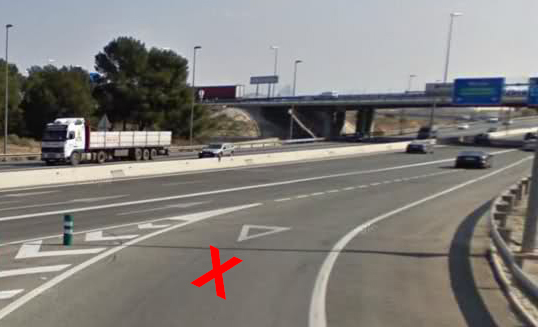
\includegraphics[width=\textwidth]{figures/3.1a.jpg}
    \caption{Opción 1}
    \label{fig:3.1a}
  \end{subfigure}
  \hfill
  \begin{subfigure}[b]{0.45\textwidth}
    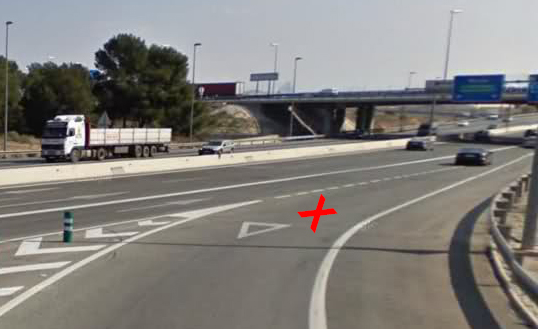
\includegraphics[width=\textwidth]{figures/3.1b.jpg}
    \caption{Opción 2}
    \label{fig:3.1b}
  \end{subfigure}
  \begin{subfigure}[b]{0.45\textwidth}
    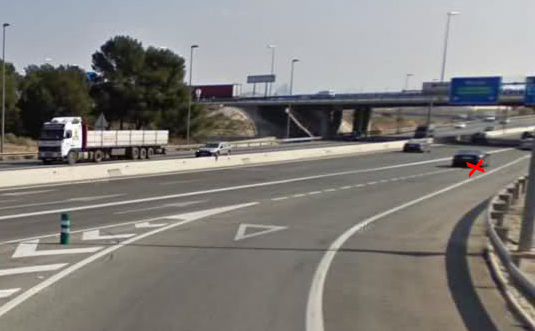
\includegraphics[width=\textwidth]{figures/3.1c.jpg}
    \caption{Opción 3}
    \label{fig:3.1c}
  \end{subfigure}
  \caption{Carril de aceleración, (a) antes de la señal, (b) después de la señal y (c) final del carril}
  \label{fig:3.1}
\end{figure}

Aproximadamente la mitad de los conductores, aun cuando se encontraron con un carril de incorporación corto y no viendo clara la salida, no pararían al principio del carril. Sin embargo, la mayor parte de los encuestados (más del 80\%) afirmaron que facilitarían la incorporación de los demás vehículos a la vía por la que circulan, siempre y cuando las condiciones se lo permitiesen. Por último, en una incorporación los conductores tendieron a fijarse en los vehículos que circulan dentro de la vía, en el vehículo que se encontrase delante y en la longitud del carril de aceleración. 

\subsubsection{3.1.1.3 Discusión}\label{3113}

Los resultados obtenidos de la encuesta sobre sensaciones y comportamientos en incorporaciones han permitido conocer en profundidad ciertos aspectos relacionados con el estrés durante la maniobra. Se observa que la experiencia en conducción y la edad guardan una relación lineal negativa con el estrés experimentado ante distintos escenarios de incorporación. Esto significa que existe una tendencia de los conductores más jóvenes y con menos experiencia a percibir más estrés en situaciones de incorporación a una vía. Hay que considerar que ambas variables están estrechamente ligadas, por lo que la variable experiencia es la más relevante en este contexto. 

En lo relativo a acciones, se observa que los conductores que informan de mayores niveles de estrés tienden a esperar hasta el final para frenar en las incorporaciones, son más arriesgados, comienzan prematuramente una incorporación si advierten que los vehículos que circulan detrás se van a incorporar primero y emplean el claxon en la autovía con mayor frecuencia que los no experimentan niveles altos de estrés. Por otro lado, se observa que los conductores suelen ser menos arriesgados en las incorporaciones cuando llevan a pasajeros en su vehículo. 

De manera general, se esperaban obtener mayores niveles de estrés frente a una incorporación, sin embargo, más del 70\% de los participantes informaron sentir poco o solo a veces estrés durante la maniobra. No obstante, estos niveles de estrés crecen si las condiciones de visibilidad son bajas o si llegan al final del carril sin velocidad suficiente. En esta última situación, la actitud de los conductores no es conservadora, ya que en caso de tener que detenerse, la mitad de los encuestados lo harían en el último tercio del carril, apoyando los resultados de \textcite{marczak}. A pesar de ello, también se observa una actitud colaborativa al manifestar en su mayoría que facilitarían la maniobra si las circunstancias lo permiten. 

Finalmente, se puede concluir que la incorporación es una maniobra muy intuitiva, la cual necesita práctica, y en cierta manera riesgo, ya que el conductor debe evaluar las intenciones de los demás vehículos utilizando solo la exploración visual como única fuente de información. Por todo ello es recomendable y beneficioso la integración de un sistema de ayuda a la incorporación con objeto de mejorar la seguridad y facilitar la realización de la maniobra.  

\subsection{Evaluación de variables atencionales en incorporaciones} \label{312}

El comportamiento visual está íntimamente ligado a la actividad cognitiva. Variables como la dirección de la mirada, las fijaciones y sacadas proporcionan información sobre la atención de la persona, pero también sobre la carga mental o el estrés, especialmente la dilatación pupilar. La complejidad de la situación tiene una relación directa con el diámetro de la pupila (\cite{wickens}; \cite{poock}), como es el ejemplo de la incorporación a una vía, donde se requiere procesar una alta cantidad de información. 

Para evaluar de manera objetiva la carga mental generada en el conductor por las situaciones de incorporación, se analiza el comportamiento visual de varios sujetos durante dicha maniobra en tráfico real, con el objetivo de diseñar una interfaz para un sistema de asistencia al conductor que facilite su incorporación al flujo vehicular. Mediante el estudio de las variables atencionales y el análisis correspondiente, se observará una influencia significativa de la carga cognitiva en la dirección de la mirada del conductor.

\subsubsection{3.1.2.1 Metodología}\label{3121}

Los sujetos que participaron en los ensayos de conducción fueron un total de 8, siendo 6 de ellos hombres y 2 mujeres. La edad y la experiencia de los participantes fue muy similar, obteniendo unos valores de 31.25 años (\emph{SD} = 4.23) para edad y 12.25 años (\emph{SD} = 4.30) para experiencia. La mayoría de los participantes manifestaron conducir de forma habitual un turismo como primer vehículo. En esta primera aproximación, el número de participantes se consideró suficiente para la obtención de resultados preliminares, los cuales fueron analizados mediante estudios estadísticos apropiados para el tamaño de la muestra. 

Los ensayos de conducción fueron realizados en un circuito en tráfico real en la zona sureste de Madrid, coincidiendo con las principales autovías M-30, M-40 y A-3 Carretera de Valencia con una duración media de 15 minutos cada uno. A lo largo de esta zona se encontraron entre 10 y 20 ocasiones donde observar situaciones de incorporación, tanto a izquierdas como a derechas gracias a los nudos entre carreteras, las cuales fueron analizadas independientemente del resto de trayecto realizado.  

Las dos condiciones principales a estudiar fueron por un lado los intervalos de incorporación y por otro, el resto del experimento, considerado como línea o tasa base. En esta última condición se instruyó a los participantes que condujeran de manera natural, obteniendo una referencia de cada uno de ellos para el análisis estadístico. Como criterio para definir el inicio de una incorporación se utilizó la primera mirada al retrovisor, ya que es en esta inspección visual donde el conductor extrajo la mayor parte de información del entorno para realizar la maniobra. El vehículo utilizado es un Peugeot 307 con cambio de marchas automático. Las respuestas oculares de los conductores han sido registradas mediante un sistema de seguimiento visual, extrayendo principalmente diámetros de pupila, fijaciones y posición en el espacio de la mirada.  
El sistema de seguimiento visual utilizado es el equipo Tobii Pro Glasses 2 (Figura \ref{fig:3.2}), cuyas ventajas frente a otros sistemas son la portabilidad y ligereza, dado que no necesita de elementos instalados permanentemente en el vehículo, la robustez ante diferencias lumínicas exteriores y la facilidad de calibración. 

\begin{figure}[h]
    \centering
    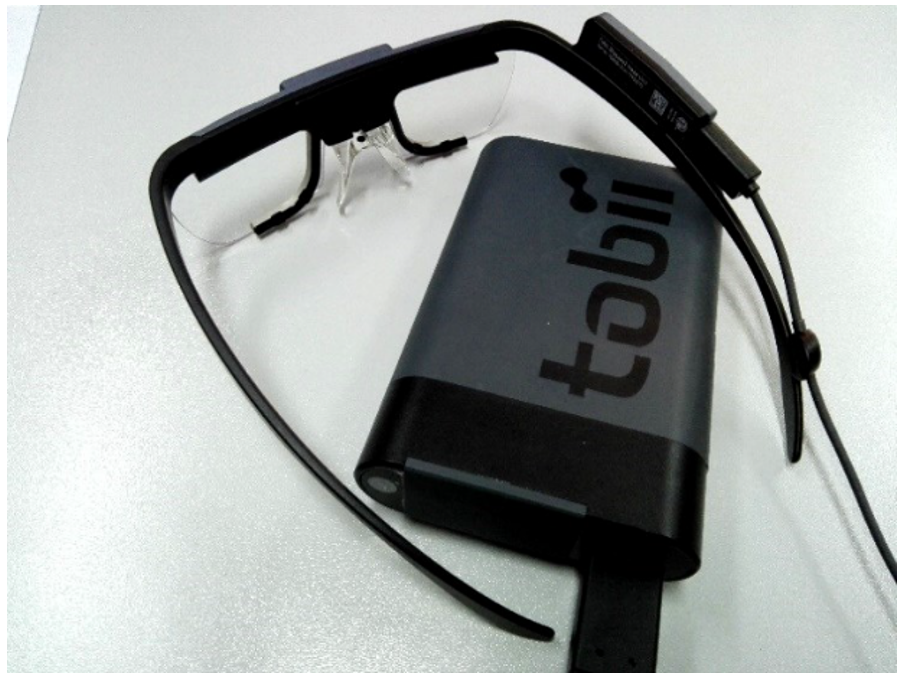
\includegraphics[width=9cm]{figures/3.2.png}
    \caption{ \label{fig:3.2} Tobii Pro Glasses 2}
\end{figure}

Las gafas están equipadas con 2 sensores infrarrojos y 4 cámaras, dos por cada ojo, permitiendo la adquisición de datos de la pupila y el comportamiento de la mirada. Además, una cámara situada en la parte delantera de las gafas adquiere información de la escena y permite ubicar la mirada del conductor en la carretera. La técnica para la detección de la mirada es el método pupila oscura, iluminando la mirada de manera no coaxial y haciendo que la pupila aparezca sombreada. El equipo se conecta mediante Ethernet al ordenador de control, capturando las siguientes variables (Tabla \ref{tab:3.2}).

Además de estas variables, se han realizado análisis de las áreas de interés durante la maniobra de incorporación y los mapas de calor de las miradas, gracias al software de la misma compañía Tobii Pro Lab.
Se han llevado a cabo análisis estadísticos no paramétricos debido al limitado tamaño de muestra empleada. Para ello se realizó la prueba de los rasgos con signo de Wilcoxon para muestras pareadas con el software SPSS v26, con objeto de comprobar si existen diferencias significativas entre ambas muestras. 

\newpage
\begin{table}[htb]
\centering
\begin{tabular}{@{}rll@{}}
\textbf{Variables}                                                                                       & \textbf{Descripción  }                                                                                                   & \textbf{Unidades}                                                                                              \\ \midrule
\begin{tabular}[c]{@{}r@{}}Dirección de la Mirada\\ (Izquierda y derecha)\end{tabular} & Dirección de la mirada en ambos ojos                                                                            & Milímetros                                                                                            \\ \midrule
Posición de la mirada 2D                                                               & \begin{tabular}[c]{@{}l@{}}Posición de la mirada dentro de los \\   límites del marco de grabación\end{tabular} & \begin{tabular}[c]{@{}l@{}}Arriba-izquierda {[}0, 0{]}\\ Abajo- derecha {[}1, 1{]}\end{tabular} \\ \midrule
Posición de la mirada 3D                                                              & La posición de la pupila en un espacio 3D                                                                       & Milímetros                                                                                            \\ \midrule
\begin{tabular}[c]{@{}r@{}}Diámetro de la pupila\\ (Izquierda y derecha)\end{tabular}  & Diámetro de la pupila en ambos ojos                                                                             & Milímetros                                                                                            \\ \midrule
\begin{tabular}[c]{@{}r@{}}Centro de la pupila  \\  (Izquierda y derecha)\end{tabular} & Centro de la pupila en ambos ojos                                                                               & Milímetros                                                                                            \\ \midrule
Giróscopo                                                                             & Velocidad angular en cada uno de los tres   ejes                                                                & °/s                                                                                                   \\ \midrule
Acelerómetro                                                                           & \begin{tabular}[c]{@{}l@{}}Aceleración de cada una de las tres \\   direcciones espaciales\end{tabular}         & m/s²                                                                                                  \\ \midrule
Vídeo                                                                                  & Grabación del ensayo                                                                                            & \begin{tabular}[c]{@{}l@{}}1920 x 1080 píxeles a \\ 25 fps\end{tabular}                               \\ \midrule
Frecuencia de muestreo                                                                 &                                                                                                                 & 50 Hz                                                                                                 \\ \bottomrule
\end{tabular}
\caption{Variables del sistema de seguimiento visual Tobii Pro Glasses 2}
\label{tab:3.2}
\end{table}

\subsubsection{3.1.2.2 Resultados}\label{3122}

\textbf{\emph{Diámetro de las pupilas}}

La mayoría de los diámetros de las pupilas de los conductores mostraron sensibilidad en las situaciones de incorporación a vías principales, aumentando su valor respecto a la línea base obtenida en conducción normal, marcado con color azul en la tabla \ref{tab:3.3}. 

\begin{table}[htb]
\centering
\begin{tabular}{@{}cccccccccll@{}}
                                            & \multicolumn{10}{c}{\textbf{Diámetro de la pupila (mm)}}                                                                                                                                                                                                                                                                                  \\ \cmidrule(l){2-11} 
                                            & \multicolumn{4}{c|}{Incorporaciones}                                                                                                                                & \multicolumn{6}{c}{Tasa   base}                                                                                                                                     \\ \cmidrule(l){2-11} 
                                            & \multicolumn{2}{c|}{\textit{Ojo Izq.}}                                           & \multicolumn{2}{c|}{\textit{Ojo   Dcho.}}                                        & \multicolumn{2}{c}{\textit{Ojo   Izq.}}                                          & \multicolumn{4}{c}{\textit{Ojo   Dcho.}}                                         \\ \cmidrule(l){2-11} 
\multirow{-4}{*}{\textbf{Sujetos}} & \textit{M}                   & \multicolumn{1}{c|}{\textit{SD}}                  & \textit{M}                   & \multicolumn{1}{c|}{\textit{SD}}                  & \textit{M}                   & \multicolumn{1}{c|}{\textit{SD}}                  & \textit{M}                    & \multicolumn{3}{c}{\textit{SD}}                  \\ \cmidrule(l){2-11} 
{A}                                  & \cellcolor[HTML]{BDD6EE}2.71 & \multicolumn{1}{c|}{\cellcolor[HTML]{BDD6EE}0.30} & \cellcolor[HTML]{BDD6EE}2.70 & \multicolumn{1}{c|}{\cellcolor[HTML]{BDD6EE}0.28} & 2.63                         & \multicolumn{1}{c|}{0.26}                         & 2.57                          & \multicolumn{3}{c}{0.27}                         \\ \midrule
{B}                                  & 1.87                         & \multicolumn{1}{c|}{0.18}                         & 1.83                         & \multicolumn{1}{c|}{0.15}                         & \cellcolor[HTML]{BDD6EE}1.89 & \multicolumn{1}{c|}{\cellcolor[HTML]{BDD6EE}0.17} & \cellcolor[HTML]{BDD6EE}1.88  & \multicolumn{3}{c}{\cellcolor[HTML]{BDD6EE}0.16} \\ \midrule
{C}                                  & \cellcolor[HTML]{BDD6EE}2.42 & \multicolumn{1}{c|}{\cellcolor[HTML]{BDD6EE}0.22} & \cellcolor[HTML]{BDD6EE}2.34 & \multicolumn{1}{c|}{\cellcolor[HTML]{BDD6EE}0.24} & 2.32                         & \multicolumn{1}{c|}{0.16}                         & 2.26                          & \multicolumn{3}{c}{0.18}                         \\ \midrule
{D}                                  & \cellcolor[HTML]{BDD6EE}2.49 & \multicolumn{1}{c|}{\cellcolor[HTML]{BDD6EE}0.23} & \cellcolor[HTML]{BDD6EE}2.56 & \multicolumn{1}{c|}{\cellcolor[HTML]{BDD6EE}0.25} & 2.46                         & \multicolumn{1}{c|}{0.27}                         & 2.45                          & \multicolumn{3}{c}{0.30}                         \\ \midrule
{E}                                  & \cellcolor[HTML]{BDD6EE}3.49 & \multicolumn{1}{c|}{\cellcolor[HTML]{BDD6EE}1.36} & \cellcolor[HTML]{BDD6EE}3.47 & \multicolumn{1}{c|}{\cellcolor[HTML]{BDD6EE}1.30} & 2.41                         & \multicolumn{1}{c|}{1.23}                         & 2.43                          & \multicolumn{3}{c}{1.22}                         \\ \midrule
{F}                                  & \cellcolor[HTML]{BDD6EE}2.48 & \multicolumn{1}{c|}{\cellcolor[HTML]{BDD6EE}0.31} & \cellcolor[HTML]{BDD6EE}2.46 & \multicolumn{1}{c|}{\cellcolor[HTML]{BDD6EE}0.29} & 2.29                         & \multicolumn{1}{c|}{0.36}                         & 2.24                          & \multicolumn{3}{c}{0.19}                         \\ \midrule
G                                           & \cellcolor[HTML]{BDD6EE}2.10 & \multicolumn{1}{c|}{\cellcolor[HTML]{BDD6EE}0.20} & \cellcolor[HTML]{BDD6EE}2.09 & \multicolumn{1}{c|}{\cellcolor[HTML]{BDD6EE}0.22} & 1.96                         & \multicolumn{1}{c|}{0.17}                         & 1.96                          & \multicolumn{3}{c}{0.17}                         \\ \midrule
H                                           & \cellcolor[HTML]{BDD6EE}1.87 & \multicolumn{1}{c|}{\cellcolor[HTML]{BDD6EE}0.20} & \cellcolor[HTML]{BDD6EE}1.85 & \multicolumn{1}{c|}{\cellcolor[HTML]{BDD6EE}0.15} & 1.83                         & \multicolumn{1}{c|}{0.16}                         & 1.77                          & \multicolumn{3}{c}{0.16}                        
\end{tabular}
\caption{Media y desviación típica del diámetro de la pupila}
\label{tab:3.3}
\end{table}

Este incremento puede verse en términos porcentuales en la figura \ref{fig:3.3}, donde la mayoría de los participantes tuvieron un aumento en la media pupilar durante la incorporación respecto a la tasa base. Excluyendo los valores atípicos se puede resumir que el diámetro pupilar aumentó aproximadamente un 5.3\% para el ojo derecho y un 4.13\% para el ojo izquierdo durante la maniobra de incorporación.

\begin{figure}[h]
    \centering
    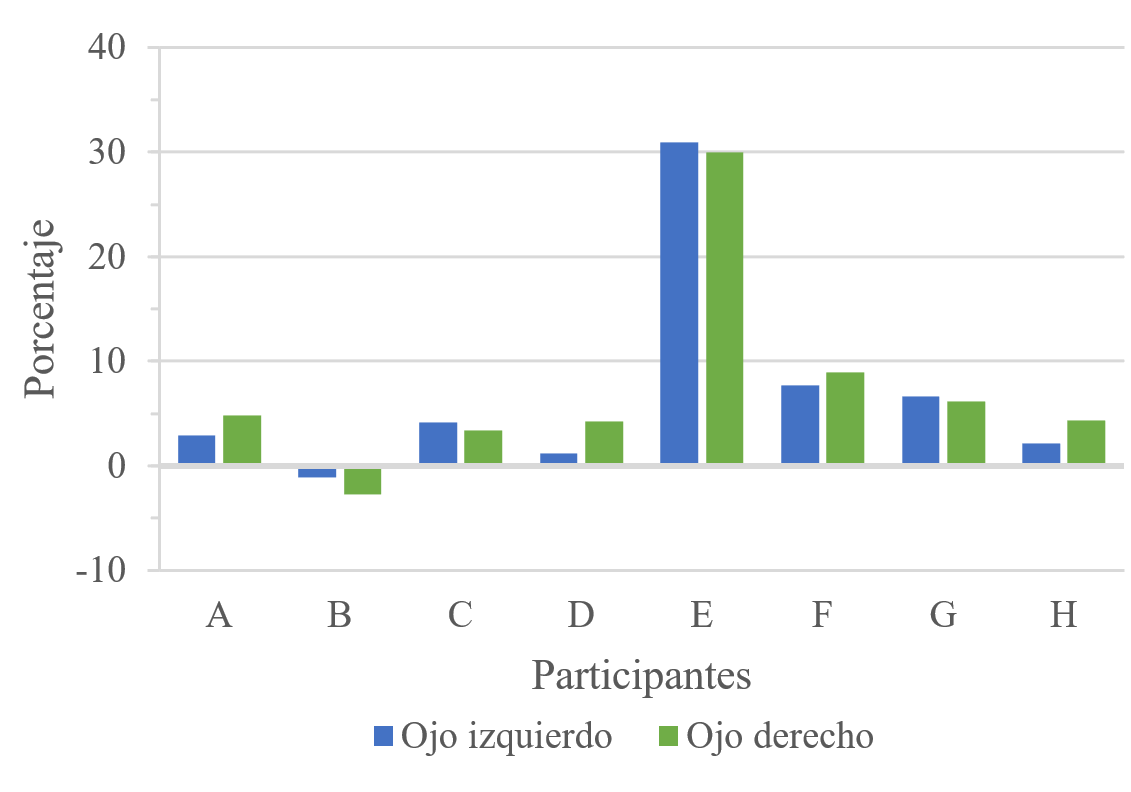
\includegraphics[width=12cm]
    {figures/3.3.png}
    \caption{ \label{fig:3.3} Porcentaje de aumento de la media pupilar en incorporaciones}
\end{figure}

A nivel estadístico se realizó una prueba de Wilcoxon, obteniendo diferencias significativas tanto para la pupila izquierda (\emph{Z} = 2.1, \emph{p} = 0.036) como en la pupila derecha (\emph{Z} = 2.38, \emph{p} = 0.016) entre las situaciones de incorporación y tasa base. 

\textbf{\emph{Fijaciones}}

Los datos obtenidos de las fijaciones permitieron realizar diferentes análisis donde observar el efecto de una incorporación en el comportamiento visual los conductores. Se han examinado los momentos de incorporación frente al resto del ensayo, y posteriormente, la influencia de los espejos retrovisores durante la maniobra.
En la duración de las fijaciones en incorporaciones frente a tasa base no se encontraron resultados significativos, ni una tendencia remarcable como se puede observar en la tabla \ref{tab:3.4}. Estos resultados son debido a la variabilidad que existe entre las diferentes áreas observadas durante una incorporación, reflejada además en los valores de desviación típica.

\newpage
\begin{table}[h]
\centering
\begin{tabular}{@{}cccccccccll@{}}
\multirow{5}{*}{\textbf{Sujetos}} & \multicolumn{10}{c}{\textbf{Duración de las fijaciones (ms)}}                       \\ \cmidrule(l){2-11} 
                                           & \multicolumn{2}{c|}{Incorporaciones}                      & \multicolumn{2}{c}{Tasa   base}                                  \\ \cmidrule(l){2-11} 
                                           & \textit{M} & \multicolumn{1}{c|}{\textit{SD}} & \textit{M} & \multicolumn{1}{c}{\textit{SD}} \\ \cmidrule(l){2-11} 
{A}                                 & 551.83     & \multicolumn{1}{c|}{783.51}      & 462.36     & \multicolumn{1}{c}{517.23}      \\ \midrule
{B}                                 & 382.17     & \multicolumn{1}{c|}{355.14}      & 342.68     & \multicolumn{1}{c}{548.21}      \\ \midrule
{C}                                 & 551.83     & \multicolumn{1}{c|}{783.51}      & 398.82     & \multicolumn{1}{c}{374.64}      \\ \midrule
{D}                                 & 210.30     & \multicolumn{1}{c|}{188.11}      & 341.80     & \multicolumn{1}{c}{455.22}     \\ \midrule
{E}                                 & 171.86     & \multicolumn{1}{c|}{131.30}      & 257.90     & \multicolumn{1}{c}{221.65}       \\ \midrule
{F}                                 & 1850.88    & \multicolumn{1}{c|}{1894.98}     & 787.44     & \multicolumn{1}{c}{1059.73}       \\ \midrule
G                                   & 294.61     & \multicolumn{1}{c|}{262.47}      & 299.20     & \multicolumn{1}{c}{252.75}     \\ \midrule
H                                   & 282.59     & \multicolumn{1}{c|}{374.36}      & 291.56     & \multicolumn{1}{c}{244.35}       \\ \midrule
\end{tabular}
\caption{Media y desviación típica de la duración de las fijaciones}
\label{tab:3.4}
\end{table}

El siguiente análisis se particularizó al área de los espejos retrovisores, evaluando la duración y número de fijaciones a los mismos respecto a las totales realizadas durante la maniobra de incorporación en términos porcentuales. Los resultados obtenidos se resumen en la tabla \ref{tab:3.5}, diferenciando entre incorporación a izquierdas y derechas.

\begin{table}[htbp]
\centering
\begin{tabular}{@{}ccc|cc@{}}
\multirow{2}{*}{\textbf{Sujetos}} & \multicolumn{2}{c|}{\textbf{\begin{tabular}[c]{@{}c@{}}\% Duración fijaciones en espejos \\ retrovisores respecto al total\end{tabular}}} & \multicolumn{2}{c}{\textbf{\begin{tabular}[c]{@{}c@{}}\% Número fijaciones en espejos \\ retrovisores respecto al total\end{tabular}}} \\ \cmidrule(l){2-5} 
                                  & \textit{Espejo   Izq.}                                              & \textit{Espejo   Dcho.}                                             & \textit{Espejo   Izq.}                                            & \textit{Espejo   Dcho.}                                            \\ \cmidrule(l){2-5} 
{A}                        & 44.46                                                               & 37.44                                                               & 45.7                                                              & 40.44                                                              \\ \midrule
{B}                        & 21.39                                                               & 21.76                                                               & 22.48                                                             & 19.86                                                              \\ \midrule
{C}                        & 36.33                                                               & 58.91                                                               & 53.37                                                             & 50.87                                                              \\ \midrule
{D}                        & 13.81                                                               & 38.02                                                               & 16.8                                                              & 37.34                                                              \\ \midrule
{E}                        & 7.56                                                                & 17.31                                                               & 18.48                                                             & 36.67                                                              \\ \midrule
{F}                        & 0                                                                   & 46.76                                                               & 0                                                                 & 33.82                                                              \\ \midrule
{G}                        & 39.16                                                               & 48.62                                                               & 16.8                                                              & 47.82                                                              \\ \midrule
{H}                        & 31.36                                                               & 42.99                                                               & 33.75                                                             & 37.66                                                              \\ \midrule
{Media total}              & 24.26                                                               & 38.98                                                               & 25.92                                                             & 38.06                                                              \\ \bottomrule
\end{tabular}
\caption{Porcentaje de duración de las fijaciones en los espejos retrovisores}
\label{tab:3.5}
\end{table}

De manera general se aprecia que las miradas a los espejos constituyen aproximadamente un 30\% de las totales respecto al resto de elementos observados en una incorporación, como pueden ser el panel de mandos, el propio carril, los carriles adyacentes o el espejo interior.  Diferenciando entre incorporación a izquierdas o a derechas, se puede observar que, en su mayoría, los valores de duración de las fijaciones y número de fijaciones son más grandes hacia derechas que hacía izquierdas en la mayoría de los participantes.

\newpage
\textbf{\emph{Mapas de calor y áreas de interés}}

En un análisis más focalizado en la maniobra de incorporación se evaluó la mirada del conductor hacia las principales áreas de interés de su entorno. De cada maniobra, se generó el mapa de calor correspondiente a la ubicación de las miradas en el habitáculo, siendo más intensas las zonas con más densidad de miradas. En las siguientes imágenes se pueden observar dos ejemplos de mapas de calor en situaciones de incorporación hacia el carril izquierdo (Figura \ref{fig:3.4a}) y hacia el carril derecho (Figura \ref{fig:3.4b}).

\begin{figure}[h]
  \centering
  \begin{subfigure}[b]{0.45\textwidth}
    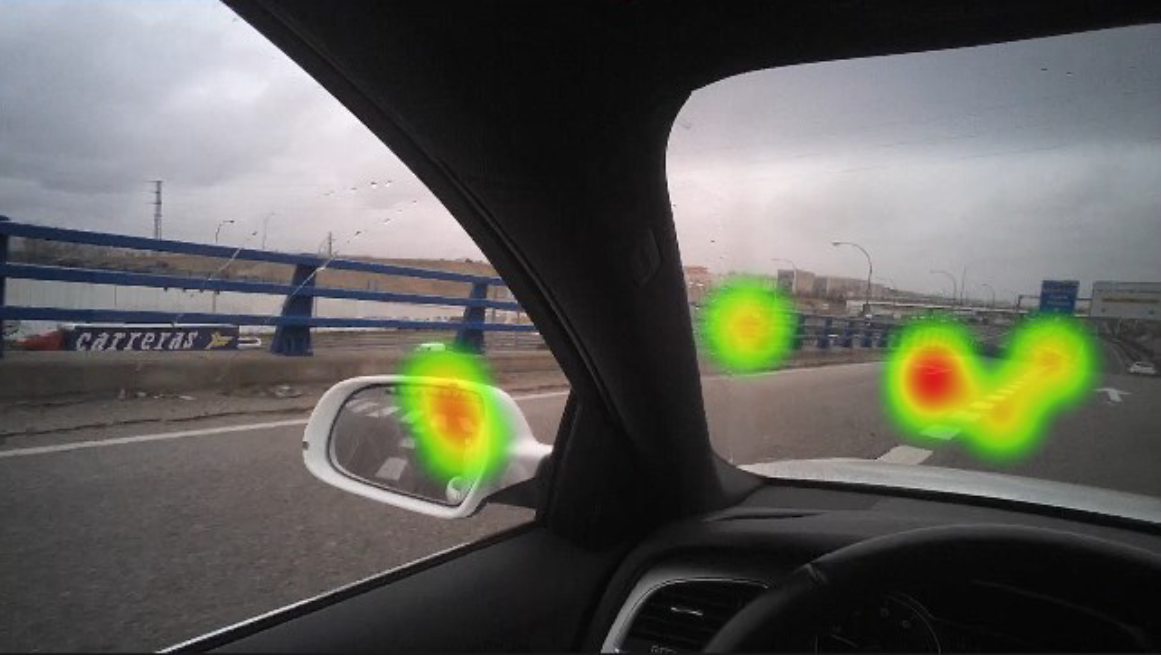
\includegraphics[width=\textwidth]{figures/3.4a.png}
     \caption{}\label{fig:3.4a}
  \end{subfigure}
  \hfill
  \begin{subfigure}[b]{0.45\textwidth}
    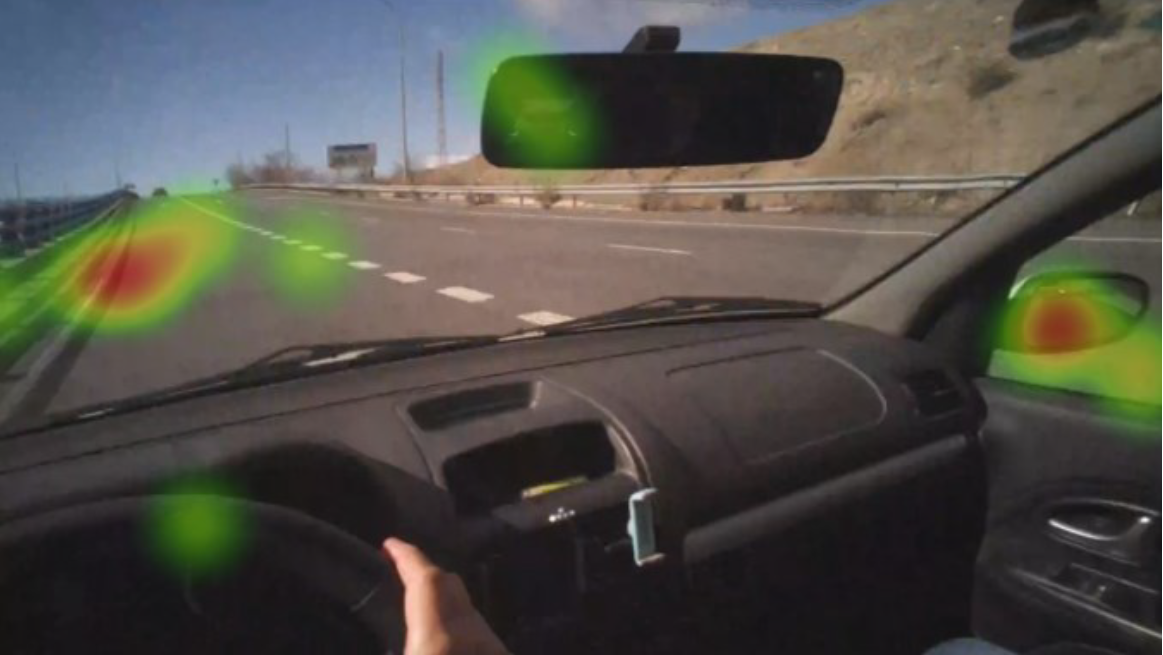
\includegraphics[width=\textwidth]{figures/3.4b.png}
     \caption{}\label{fig:3.4b}
  \end{subfigure}
  \caption{Mapas de calor de la actividad visual: (a) en incorporación hacia el carril izquierdo, (b) en incorporación hacia el carril derecho}
  \label{fig:3.4}
\end{figure}

En la mayoría de los mapas analizados de todos los participantes, es destacable un punto caliente común a ambos espejos retrovisores en la zona superior-interior del cristal, como se aprecia en las anteriores imágenes. 
En el análisis de las áreas de interés, se ha segmentado la imagen en las siguientes zonas: coche/salpicadero, señal, carril central, carril derecho, carril izquierdo, espejo retrovisor derecho, espejo retrovisor izquierdo y espejo interior (Figuras \ref{fig:3.5a} y \ref{fig:3.5b}). Cabe destacar que, debido a la escasez de datos, las medidas tomadas de las áreas señales, carril derecho, espejo retrovisor derecho y espejo interior han sido excluidas del análisis. 

\begin{figure}[h]
  \centering
  \begin{subfigure}[b]{0.45\textwidth}
    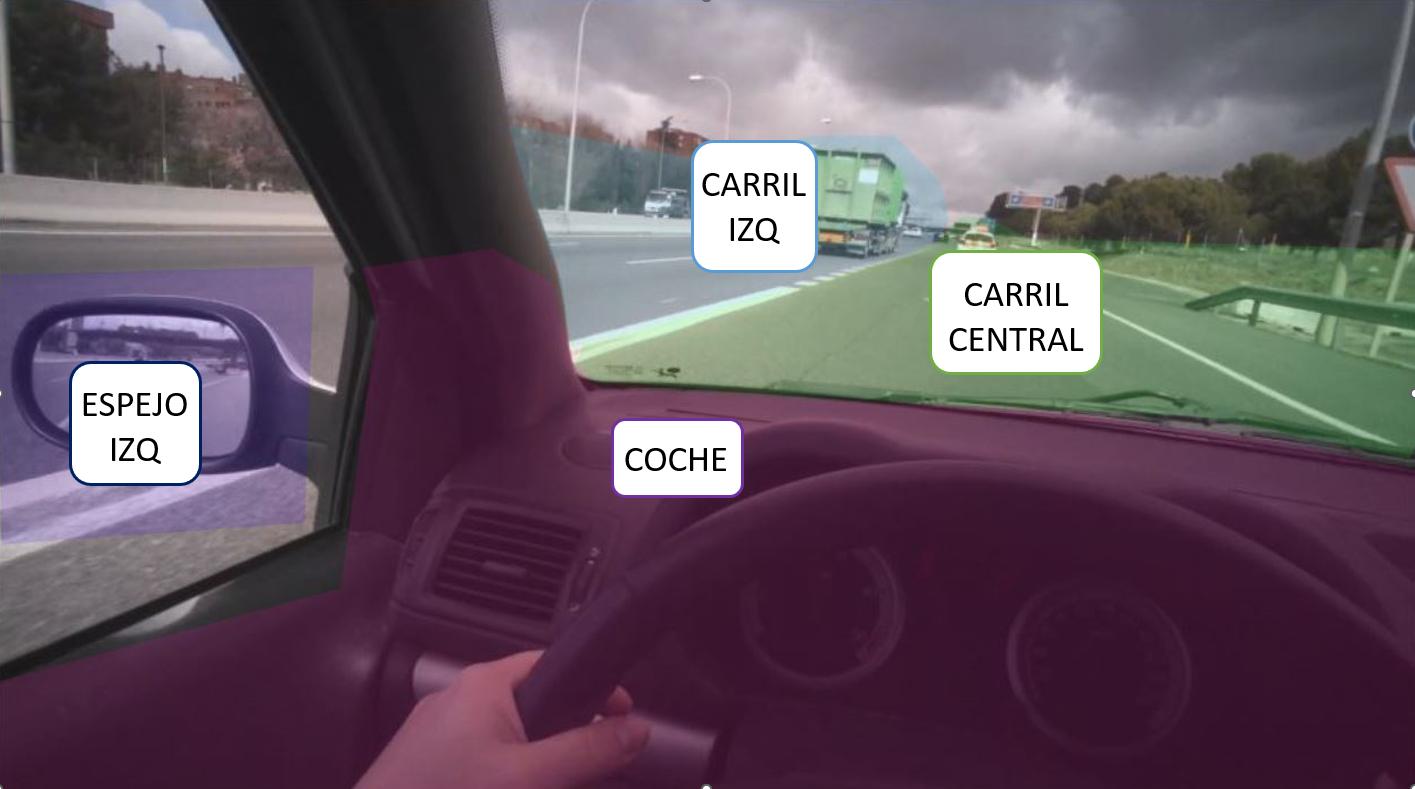
\includegraphics[width=\textwidth]{figures/3.5a.png}
    \caption{}\label{fig:3.5a}
  \end{subfigure}
  \hfill
  \begin{subfigure}[b]{0.45\textwidth}
    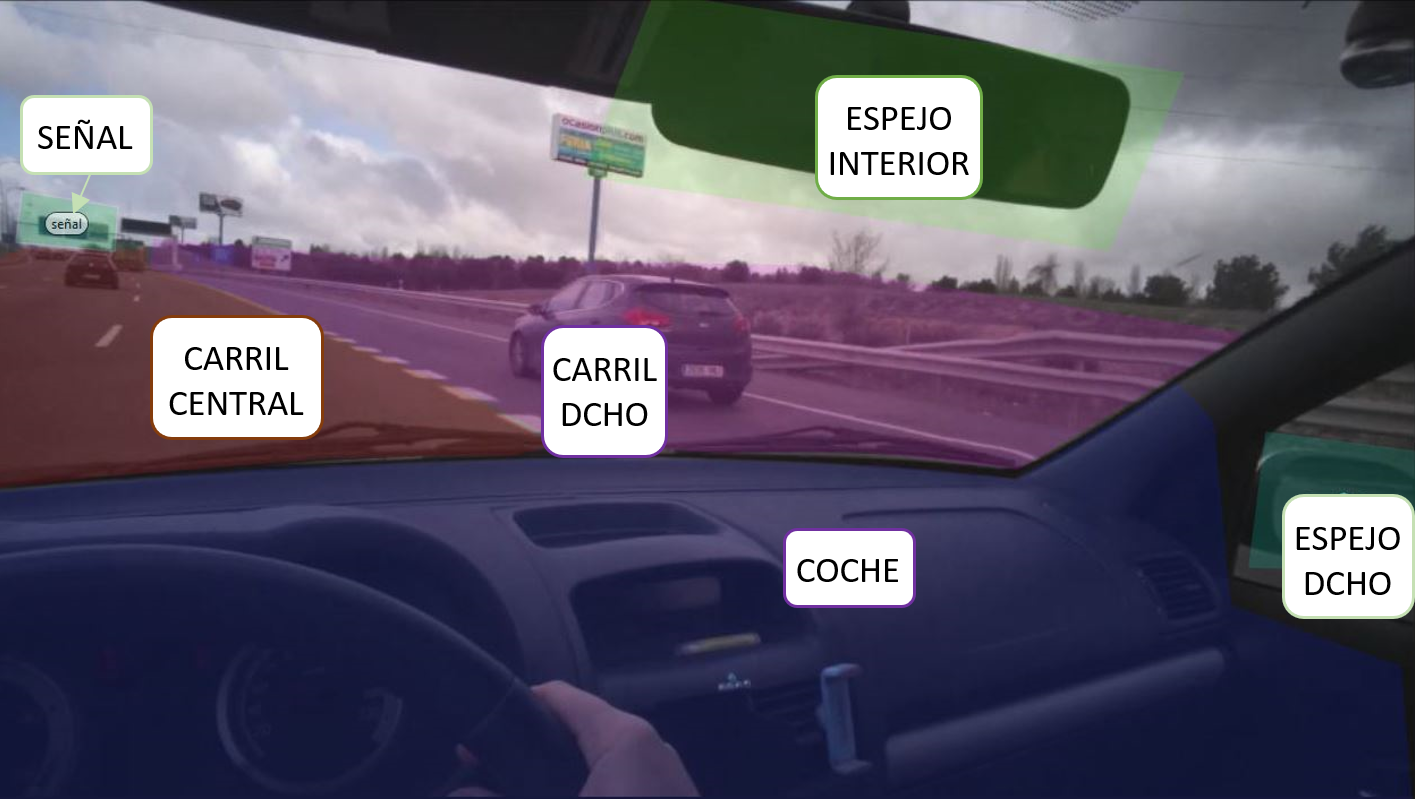
\includegraphics[width=\textwidth]{figures/3.5b.png}
    \caption{}\label{fig:3.5b}
  \end{subfigure}
  \caption{Segmentación de áreas de interés: (a) en incorporación hacia el carril izquierdo, (b) en incorporación hacia el carril derecho}
  \label{fig:3.5}
\end{figure}

Las variables a estudiar fueron la duración total de las fijaciones, el número total de fijaciones y la duración de la primera fijación en el área. Una prueba no paramétrica de Wilcoxon para hallar diferencias significativas entre el periodo de incorporación y la tasa base de cada zona, se realizó sobre cada uno de estos tres parámetros, obteniendo resultados desde tres puntos de vista diferentes. Dado que no todas las incorporaciones duraron lo mismo, se han reformulado los datos tomados expresándolos en relación con intervalo de tiempo que duró el evento. Posteriormente, se han mediado los valores correspondientes a las incorporaciones y a la tasa base de cada sujeto, obteniendo así una pareja de valores por participante. En la tabla \ref{tab:3.6} se muestran los resultados de la prueba no paramétrica, donde se observan las diferencias significativas en las medianas de los tres parámetros propuestos para cada área de interés, comparando entre situación de tasa base e incorporación.

\begin{table}[ht]
\centering
\resizebox{\textwidth}{!}{%
\begin{tabular}{cccc}
\textbf{Áreas de interés} & \textbf{\begin{tabular}[c]{@{}c@{}}Duración de\\ fijaciones / segundo\end{tabular}} & \textbf{\begin{tabular}[c]{@{}c@{}}Número de \\ fijaciones / segundo\end{tabular}} & \textbf{\begin{tabular}[c]{@{}c@{}}Duración de la primera \\ fijación / segundo\end{tabular}} \\ \hline
{Carril   central}          & \begin{tabular}[c]{@{}c@{}}Si   (línea base alta, \\ \emph{p} = 0.018)\end{tabular}      & No                                                                                 & \begin{tabular}[c]{@{}c@{}}Si   (línea base baja, \\ \emph{p} = 0.018)\end{tabular}                  \\ \hline
{Carril   izquierdo}        & No                                                                                & No                                                                                 & \begin{tabular}[c]{@{}c@{}}Si   (línea base baja, \\ \emph{p} = 0.018)\end{tabular}                  \\ \hline
{Espejo   izquierdo}        & \begin{tabular}[c]{@{}c@{}}Si   (línea base baja, \\ \emph{p} = 0.018)\end{tabular}      & \begin{tabular}[c]{@{}c@{}}Si   (línea base baja,   \\  \emph{p}   = 0.018)\end{tabular}  & \begin{tabular}[c]{@{}c@{}}Si   (línea base baja, \\ \emph{p} = 0.028)\end{tabular}                  \\ \hline
{Coche/Salpicadero}         & No                                                                                & No                                                                                 & No                                                                                            \\ \hline
\end{tabular}%
}
\caption{Diferencias significativas entre tasa base e incorporación en las áreas de interés}
\label{tab:3.6}
\end{table}
 
Los resultados más destacables se observan en la duración de la primera fijación, el cual fue superior en escenarios de incorporación para casi todas las áreas de interés, debido al análisis de la situación previo a la realización de la maniobra. En el espejo izquierdo todas las variables de seguimiento visual analizadas fueron superiores durante la incorporación, reforzando los resultados previamente obtenidos en las fijaciones y los mapas de calor. Contrariamente, el carril central se obtuvo una duración de las fijaciones mayor durante la tasa base, dado que durante una conducción crucero el conductor fija toda su atención en esta área. 

Por último, se analizaron de nuevo las diferencias significativas entre áreas durante una incorporación, en los parámetros de duración total y número de fijaciones por segundo. El parámetro de duración de la primera fijación se excluyó de este análisis debido a la escasez de datos para poder realizar la prueba estadística. Los resultados obtenidos se representan en la tabla \ref{tab:3.7}, relacionando las diferentes áreas entre sí.

\begin{table}[hb]
\centering
\resizebox{\textwidth}{!}{%
\begin{tabular}{ccc}
\textbf{Áreas de interés}                                                                & \textbf{Duración fijaciones / segundo}                                                               & \textbf{Número de fijaciones / segundo}                                                            \\ \hline
{Carril central – Carril   izq.}                                                  & \begin{tabular}[c]{@{}c@{}}Si (Carril central \textgreater   Carril izq., \\ \emph{p} = 0.028)\end{tabular} & No                                                                                                 \\ \hline
{Carril central – Espejo   izq.}                                                  & No                                                                                                   & No                                                                                                 \\ \hline
{\begin{tabular}[c]{@{}c@{}}Carril central –   \\ Coche/Salpicadero\end{tabular}} & \begin{tabular}[c]{@{}c@{}}Si (Carril central \textgreater   Coche,\\ \emph{p}   = 0.028)\end{tabular}      & \begin{tabular}[c]{@{}c@{}}Si (Carril central \textgreater   Coche,   \\ \emph{p}   = 0.028)\end{tabular} \\ \hline
{Carril izq. – Espejo   izq.}                                                     & No                                                                                                   & \begin{tabular}[c]{@{}c@{}}Si (Carril izq. \textless   Espejo izq., \\ \emph{p}   = 0.028)\end{tabular}   \\ \hline
{\begin{tabular}[c]{@{}c@{}}Carril izq. –   \\ Coche/Salpicadero\end{tabular}}    & No                                                                                                   & \begin{tabular}[c]{@{}c@{}}Si (Carril izq. \textgreater   Coche, \\ \emph{p}   = 0.043)\end{tabular}      \\ \hline
{\begin{tabular}[c]{@{}c@{}}Espejo izq. – \\ Coche/Salpicadero\end{tabular}}      & \begin{tabular}[c]{@{}c@{}}Si (Espejo izq. \textgreater Coche, \\ \emph{p}   = 0.028)\end{tabular}          & \begin{tabular}[c]{@{}c@{}}Si (Espejo izq. \textgreater Coche, \\ \emph{p}   = 0.018)\end{tabular}        \\ \hline
\end{tabular}%
}
\caption{Diferencias significativas en duración y número de fijaciones por segundo entre áreas de interés}
\label{tab:3.7}
\end{table}

\newpage
Se observa que el área con menos diferencias entre la situación de incorporación y la tasa base fue el área coche o salpicadero, no apareciendo como la variable más alta en ninguna de las comparaciones de las dos tablas. No obstante, en el área espejo izquierdo y carril central se obtuvieron valores más altos durante la incorporación en ambas tablas, duración y número de fijaciones, siendo estas zonas muy observadas por conductor en la realización de la maniobra. 

\subsubsection{3.1.2.3	Discusión}\label{3123}

En este estudio se ha analizado la influencia de las variables atencionales de un conductor durante la maniobra de incorporación en tráfico real. A través de un sistema de seguimiento visual, se han obtenido diferencias significativas en ambas dilataciones pupilares, aumentando su valor alrededor de un 5\% durante la incorporación frente a la tasa base. 

Sin embargo, este resultado no se ve replicado en la duración de las fijaciones representada en la tabla  \ref{tab:3.5}, las cuales sí revelaron que aproximadamente un 30\% de las mismas se hacían a los espejos retrovisores en comparación con el resto de elementos que son observados durante una incorporación, como son el panel de mandos, el carril central, carriles adyacentes o el espejo interior. Este valor pone de manifiesto la importancia en el diseño y el uso de los espejos retrovisores, dado que gran parte del tiempo es dedicado a la exploración del entorno a través de ellos para poder realizar una maniobra lo más segura posible.

En relación con las fijaciones a los dos espejos retrovisores (Tabla \ref{tab:3.5}) se observó que, tanto la duración de las fijaciones como el número de las mismas, fueron más frecuentes a derechas que a izquierdas, pudiendo deberse a diferentes razones. Por un lado, en las incorporaciones a izquierdas se observó un mayor uso del espejo interior como complemento al espejo izquierdo, dando como resultado menores fijaciones al espejo izquierdo en comparación con el derecho. Por otro, este fenómeno también podría estar relacionado con la inseguridad y falta de hábito por parte de los conductores de realizar una incorporación a derechas, ya que la más común es a izquierdas y tiene una estructura muy similar a la maniobra de cambio de carril. Además, las incorporaciones a derechas requieren un giro de la cabeza más amplio, siendo este movimiento poco natural para el conductor. Un mayor tiempo en las fijaciones puede ser interpretado como una exploración en profundidad del entorno debido a su complejidad. El mismo efecto puede ser observado con un mayor número de fijaciones aun siendo su duración menor, ya que un número alto de fijaciones señala la necesidad de volver a explorar la situación.

En los mapas de calor se observó un punto caliente interesante en la esquina superior-interior del espejo, común a ambos retrovisores. Este resultado revela la gestión atencional de los conductores ante la demanda cognitiva de la situación de incorporación. Se puede concluir que la elección de esta zona es debido a que no está demasiado alejada del centro de la calzada, pero a su vez aporta suficiente información del carril lateral gracias a la visión periférica. Esta zona se considera interesante para la ubicación de futuras interfaces de ayuda a la conducción.

En el análisis de las áreas de interés se encontraron limitaciones del sistema, debiendo postprocesar parte de los datos manualmente. En los ensayos se advirtió que algunos conductores realizaron movimientos corporales y giros de cabeza bastante bruscos y frecuentes, especialmente cuando se miraba al espejo retrovisor derecho y en las incorporaciones a una vía. A pesar de que el sistema de adquisición dispone de un giróscopo y un acelerómetro para determinar el movimiento de la cabeza del conductor, y por tanto la dirección de su mirada, la propia deriva característica de los sensores junto a la longitud de los ensayos de conducción supuso la aparición de un error acumulativo. En consecuencia y para asegurar una buena calidad de los resultados, se suprimió dicha fuente de datos y se palió mediante una codificación manual de las áreas y los giros de la cabeza. En el siguiente capítulo se presenta una solución de bajo costo que resuelve de forma automática dichos inconvenientes. 

Los resultados mostraron la importancia de la primera fijación en todas las áreas de interés, evidenciando resultados estadísticamente significativos entre la tasa base y la incorporación. Como se presuponía, las primeras fijaciones durante una incorporación son más largas que en el periodo de tasa base, debido a la gran cantidad de información del entorno necesaria para la toma de decisiones. Por otro lado, también se advierte una mayor duración y número de fijaciones en el espejo izquierdo durante la incorporación, siendo este resultado coherente con los obtenidos en los mapas de calor, porcentaje de fijaciones en los espejos y diámetro de la pupila. 

Con respecto al carril central, la duración de las fijaciones es mayor en la tasa base que en la incorporación, a diferencia de otras zonas. Este resultado tiene mucho sentido, ya que en conducción normal el conductor centra la mayor parte de su atención en el obstáculo que se encuentra frente a su vehículo. 

En la comparación entre áreas de interés durante la maniobra de incorporación se observó que la zona del coche o salpicadero fue la que menos fijaciones en duración y número obtuvo, a diferencia del espejo izquierdo y el carril central. Este resultado se muestra en la tabla \ref{tab:3.7} donde no aparece en ningún caso como la variable más alta. La información que proporciona esta zona no es consideraba relevante en una situación de incorporación, todo lo contrario que la que se adquiere del espejo izquierdo, donde sí hay diferencias significativas tanto en duración como en número de fijaciones respecto al coche/salpicadero. De la misma forma, también se aprecian diferencias entre el carril central y el coche/salpicadero, viéndose reforzada la afirmación anterior.

En el siguiente estudio se plantea una interfaz de ayuda a la conducción para situaciones de incorporación, con la expectativa de que el conductor aumente las miradas al vehículo delantero y así pueda prestar atención conjuntamente al vehículo y a la carretera. 

\subsection{Sistema de asistencia en incorporaciones y diseño de HMI}\label{313}

Las situaciones de incorporación en autovías son situaciones complejas para los conductores, los cuales deben manejar mucha información en un periodo corto de tiempo tal y como se ha visto en el apartado anterior. El sistema propuesto se basa en un estudio previo donde se desarrolló un dispositivo de adaptación inteligente de la velocidad (\cite{jimenez12}). Dicho sistema informaba al conductor sobre la velocidad que debía adquirir al llegar a un tramo de carretera y le sugería, en términos cualitativos, cuánto aumentar o disminuir su velocidad al acercarse a ese tramo. En este caso, el sistema de asistencia a la incorporación proporciona al conductor información similar sobre cómo adaptar su velocidad para incorporarse a la carretera principal. 

El funcionamiento del sistema de ayuda a las incorporaciones puede resumirse en la figura \ref{fig:3.6}, donde el vehículo 1 calcula el hueco disponible entre los vehículos 2 y 3 para realizar la maniobra, respetando siempre un margen de seguridad, \emph{T}. Si finalmente no fuera posible, recomendaría al conductor esperar para incorporarse después del vehículo 3. 

\begin{figure}[h]
    \centering
    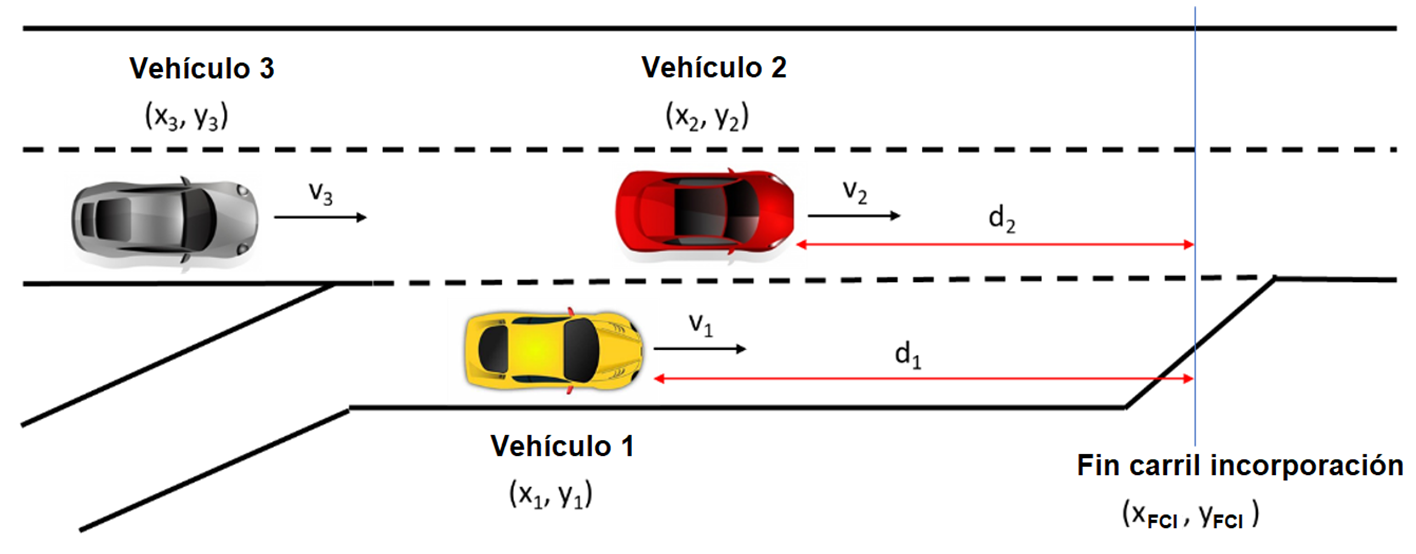
\includegraphics[width=12.5cm]
    {figures/3.6.png}
    \caption{ \label{fig:3.6} Vehículo en el carril de incorporación (vehículo 1), en la carretera principal (vehículos 2 y 3) y variables que intervienen en el algoritmo}
\end{figure}

Por otro lado, las interfaces hombre-máquina (\gls{hmi}) deben diseñarse ergonómicamente, tanto física como cognitivamente, para evitar causar distracciones al conductor.  Sin embargo, es habitual que aspectos como la usabilidad y satisfacción del usuario no sean evaluados, llevando a una mala percepción de la utilidad del sistema y por consiguiente a una pérdida de confianza y desestimación del uso del mismo. En situaciones de incorporación, el diseño de una \gls{hmi} se vuelve aún más importante, ya que la carga atencional es alta y el intervalo de tiempo para ejecutar la maniobra corto.

Este problema es abordado en \textcite{burns}, donde se resumen algunas de las características deseables en los sistemas a bordo de vehículos, como es que la duración media de la mirada a la interfaz no debe ser superior a 1.2 segundos o que el dispositivo no debe afectar al control del vehículo, ni a la carga de trabajo del conductor, ni a su conciencia situacional, atrayendo solo su atención en caso de ser necesario. En \textcite{harvey}, se enfatiza la importancia de que el dispositivo no sólo sea seguro y eficiente, sino que también sea aceptable por el usuario y su aprendizaje no requiera ninguna formación específica.

Por ello y adicionalmente, en este estudio se evalúan diferentes interfaces de asistencia al conductor para el sistema de ayuda a la incorporación. Su evaluación se realiza en un simulador de conducción, donde se proyectan grabaciones del funcionamiento del sistema real, el cual fue previamente diseñado y materializado. Se analizan los datos del simulador, del sistema de seguimiento visual de los participantes y se complementan los resultados con encuestas de aceptación y esfuerzo mental.

\subsubsection{3.1.3.1	Definición del algoritmo }\label{3131}

El diagrama de flujo presentado en la figura \ref{fig:3.7} compila la estructura del algoritmo de toma de decisiones para el sistema de ayuda a la incorporación, donde el subíndice 1 representa el vehículo que se incorpora, y 2, el vehículo que se encuentra dentro de la vía principal. 

\begin{figure}[h]
    \centering
    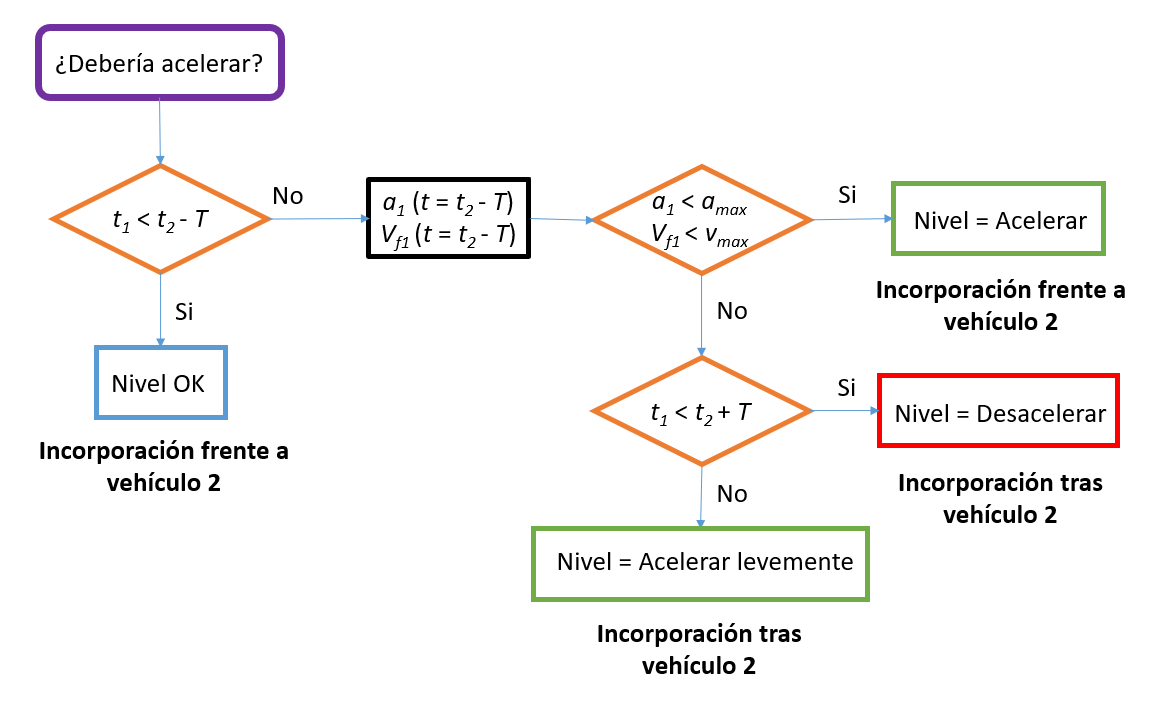
\includegraphics[width=12.5cm]
    {figures/3.7.png}
    \caption{ \label{fig:3.7} Diagrama de flujo del algoritmo de decisión}
\end{figure}

En el primer paso se evalúa si el tiempo que tarda el vehículo 1, \emph{t$_1$}, al final del carril es menor que el del vehículo 2, \emph{t$_2$}, teniendo en cuenta el margen de seguridad establecido, \emph{T}. El tiempo que tarda cada vehículo al final del carril se calcula mediante la ecuación \ref{eq:1}.

\begin{equation}\label{eq:1}
t_1 = \frac{d_i}{v_i}
\end{equation}

 En caso de que el vehículo 1 llegue antes que el vehículo 2, contando con el margen de seguridad, no será necesaria ninguna acción diferente al estado que tienen en ese instante. Si no se cumpliera esta condición, el algoritmo evaluaría si la incorporación se pudiera realizar por delante o por detrás del vehículo 2. En un primer escenario, si el vehículo 1 pudiese adquirir la aceleración necesaria, \emph{a$_1$}, sin superar la aceleración, \emph{a\textsubscript{max}}, ni la velocidad máxima de la vía, \emph{v\textsubscript{max}}, este pasaría delante del vehículo 2. La aceleración necesaria y la velocidad máxima al final del carril vienen dadas por las ecuaciones \ref{eq:2} y \ref{eq:3}.

 \begin{equation}\label{eq:2}
     a_1(t) = \dfrac{d_1-v_1\cdot t}{0.5\cdot t^2}
 \end{equation}

  \begin{equation}\label{eq:3}
      v_{f1}(t) = a_1 \cdot t + v_1
 \end{equation}

En caso contrario, la incorporación debería de hacerse detrás del vehículo 2, comprobando de nuevo la relación de tiempos al final del carril de ambos vehículos junto al margen de seguridad. En función de este resultado, el algoritmo aconsejaría realizar una desaceleración o, si hubiera suficiente distancia, recomendaría acelerar hasta un nivel máximo. Se ha de tener en cuenta que, si existiera un vehículo 3, el bucle se repetiría para verificar que la incorporación entre los vehículos es lo suficientemente segura. 

Al ser el entorno de la maniobra una vía principal tipo autovía o autopista, su velocidad está acotada legalmente a 120 km/h. Dado que a velocidades altas se requieren mayores distancias para frenar, se ha definido un margen de seguridad conservador de 2 segundos en términos de tiempo en base a investigaciones previas y valores utilizados en simuladores de conducción.  De la misma manera, los valores máximos de aceleración y deceleración se han establecido en 2 m/s$^2$ y 4 m/s$^2$ respectivamente. El algoritmo de control presentado posee una baja carga computacional, lo que hace que funcione adecuadamente en tiempo real. El código se implementa en una aplicación móvil con sistema iOS. 

Finalmente, el sistema sugiere al conductor las acciones de acelerar o frenar para realizar la maniobra con seguridad en función de las variables de los vehículos aledaños, respetando en todo momento el margen entre ellos. 

\textbf{\emph{Diseño y localización de la interfaz}}

Los diseños fueron seleccionados en base a la propia experiencia del grupo de investigación en el diseño y validación de interfaces para la conducción segura en dispositivos móviles para aplicaciones anteriores (\cite{jimenez12}; \cite{jimenez16}). Como premisa, se han seguido las Recomendaciones de la Comisión de las Comunidades Europeas de 26 de mayo de 2008, relativas a sistemas de información y comunicación a bordo de vehículos seguros y eficientes (\cite{european}). 

En la figura \ref{fig:3.8a}, se muestran las interfaces propuestas, derivando su diseño del campo de la aeronáutica, en concreto de los variómetros, y presentando la información en forma de conjunto de barras o segmentos circunferenciales. En la figura \ref{fig:3.8b} se puede observar un ejemplo de aplicación de una interfaz sobre el fondo de un navegador de conducción, soportado por un smartphone.

\newpage
\begin{figure}[htbp]
    \centering
    \begin{subfigure}[b]{0.4\linewidth}
        \centering
        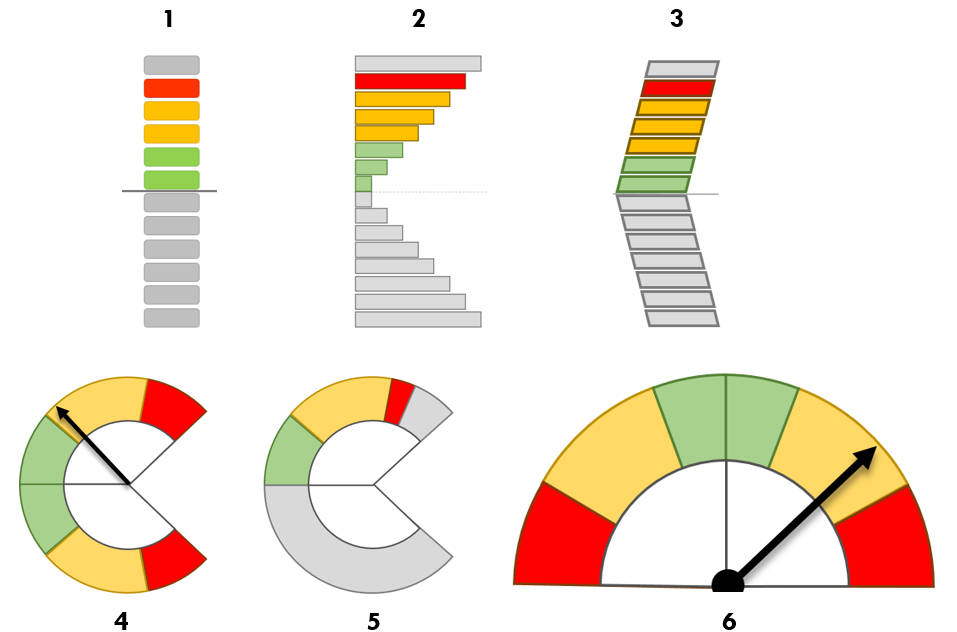
\includegraphics[width=9cm]{figures/3.8a.png}
        \caption{}
        \label{fig:3.8a}
    \end{subfigure}
    \hspace{0.5cm}
    \begin{subfigure}[b]{0.5\linewidth}
        \centering
        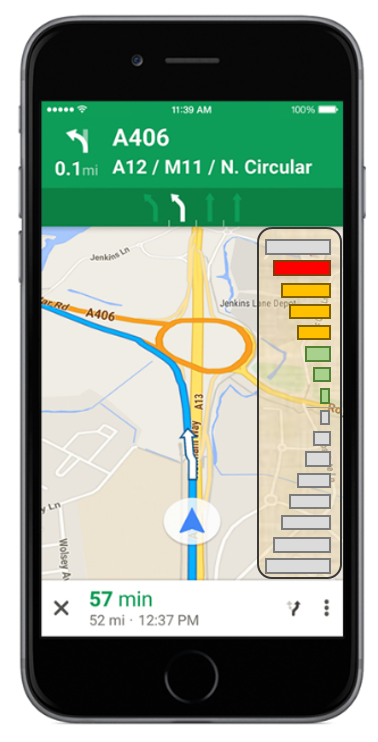
\includegraphics[width=3cm]{figures/3.8b.png}
        \caption{}
        \label{fig:3.8b}
    \end{subfigure}
     \caption{(a) Propuestas de diseños de interfaz. (b) Ejemplo de aplicación en un smartphone }
  \label{fig:3.8}
\end{figure}

La interpretación de los colores es sencilla, cuando más cerca el indicador de la zona roja o más barras aparezcan, mayor aceleración o deceleración se requerirá para realizar la maniobra con seguridad. La interfaz sea ha diseñado para ser configurable por el usuario, pudiendo elegir cuál de los extremos indica acelerar o decelerar, para un entendimiento más intuitivo. La razón de esta característica reside en los resultados obtenidos de una encuesta-sondeo sobre la interpretación de la interfaz 1, elegida por su sencillez. Los participantes contestaron a la siguiente pregunta proyectada junto a la imagen de la interfaz 1:

\emph{``Imagina que vas conduciendo por una carretera y estás a punto de incorporarte a una autopista. Dentro de tu coche se activa un dispositivo de ayuda a la incorporación que te permite conocer si vas muy rápido o muy despacio, pudiendo adecuar la velocidad de tu coche a la situación. Este dispositivo tiene en cuenta diversos factores tales como la velocidad y posición del resto de vehículos y las condiciones de la carretera. Si antes de incorporarte aparece el dispositivo de la siguiente manera, considerarías que tienes que: 1. Frenar, 2. Acelerar''}

Se obtuvieron 209 respuestas para una población de 119 hombres y 90 mujeres, con edades comprendidas de 20 a 90 años (\emph{M} = 43.39, \emph{SD} = 13.34) y una experiencia en conducción de 22.20 años (\emph{SD} = 13.53). Los resultados mostraron respuestas similares en ambas configuraciones, 46.88\% acelerar y 53.11\% frenar.
Finalmente, las interfaces seleccionadas para su evaluación fueron 1, 3 y 6, elegidas gracias al equipo de expertos pertenecientes al Departamento de  Psicobiología y Metodología en Ciencias del Comportamiento de la Universidad Complutense de Madrid. Los criterios de selección fueron los siguientes: la interfaz 1 fue elegida por su sencillez; la interfaz 3 por su similitud con la 1 y 2, además de la ventaja de poder señalar la dirección hacia donde se va a realizar la incorporación; y la interfaz 6 por su similitud con el velocímetro del cuadro de mandos de un vehículo, siendo este diseño familiar para los conductores y a la vez diferente respecto a las anteriores interfaces. 
Su localización se sitúa en la parte inferior del pilar A izquierdo, en base a los resultados obtenidos de los mapas de calor del subapartado \hyperref[3122]{3.1.2.2}.

\subsubsection{3.1.3.2	Metodología}\label{3132}

Un total de 23 sujetos, siendo 11 de ellos hombres y 12 mujeres, participaron en el estudio de evaluación de interfaces en un simulador de conducción. La edad de los participantes esta comprendidas entre los 18 y los 53 años (\emph{M} = 28, \emph{SD} = 9.4). Su experiencia media al volante fue de 8.4 años y la desviación estándar de 9.4. De manera general, los participantes declararon conducir regularmente un vehículo turismo.

El estudio de las interfaces y los ensayos en el simulador fue fruto del grupo de investigación, en colaboración con el Departamento de  Psicobiología y Metodología en Ciencias del Comportamiento de la Universidad Complutense de Madrid, donde se ubicaba el propio simulador de conducción. Dicho simulador se encuentra instalado dentro de una cabina de Faraday. Se proyectaron tres grabaciones de 5 minutos para cada una de las interfaces, donde los participantes realizaron la tarea de conducción simulada mediante un volante y un conjunto de pedales de aceleración y freno. El simulador disponía de cambio de marchas automático. 

Previo al inicio del ensayo los participantes eligieron la configuración de funcionamiento que les resultaba más intuitiva y se les pidió que condujeran de la forma más natural posible siguiendo las instrucciones de la interfaz. Al finalizar cada grabación respondieron a las encuestas de aceptación, usabilidad del sistema y esfuerzo mental sobre la interfaz. Finalmente, también respondieron a preguntas sobre información demográfica y si implementarían este sistema en su teléfono móvil si fuera gratuito.

El diseño de la investigación fue intrasujeto, donde todos los participantes pasaron por las mismas tres situaciones experimentales, una para cada tipo de interfaz, y las interfaces aparecieron de forma contrabaleanceada para paliar los efectos de orden. La duración media de cada sesión fue de 20 minutos en total. Las condiciones analizadas son las mismas que las descritas en el subapartado \hyperref[3121]{3.1.2.1.}, diferenciando los intervalos de incorporación del resto del ensayo (línea base) a raíz de la primera mirada al retrovisor. 

El análisis de la mirada también se realizó con el sistema de seguimiento ocular empleado en el subapartado \hyperref[3121]{3.1.2.1.}, adquiriendo las variables descritas anteriormente. 
Para cada interfaz se midieron las siguientes variables: A) Aceptación del sistema (Satisfacción, Utilidad y Usabilidad); B) Esfuerzo mental (a través de una medida subjetiva, la Escala de Valoración del Esfuerzo Mental (\gls{rsme}) y de la medida fisiológica de la dilatación pupilar); C) Medidas oculares (tiempo total mirando la interfaz, número y duración media de fijaciones) y medidas del seguimiento de la interfaz (porcentaje de seguimiento de la interfaz en velocidad y dirección); D) Mapas de calor.
Después de cada simulación, donde se realizaba la tarea de conducción simulada para un modelo de interfaz, los participantes respondían al cuestionario de Aceptación de Sistemas de \textcite{vanderlaan}. Este cuestionario constó de nueve ítems de 5 respuestas, que puntuaron para las escalas de utilidad del sistema y satisfacción entre -2 y +2. Posteriormente, los participantes respondieron a la Escala de Usabilidad del Sistema (\cite{brooke}), puntuada entre 0 y 100, y a la Escala de Valoración del Esfuerzo Mental \gls{rsme} (\cite{zijlstra};) cuyos valores se encuentran entre 0-150 puntos. Al final de las 3 simulaciones de conducción, también respondieron a algunas preguntas sobre información demográfica, así como si implementarían o no la aplicación en su móvil si fuera gratuita. 
Para cada diseño, se realizó un análisis de varianzas (\gls{anova}) unifactorial de medidas repetidas con el software SPSS v26. El ajuste de las comparaciones por pares se realizó mediante el método de Bonferroni. 

\subsubsection{3.1.3.3 Resultados}\label{3133}

\textbf{\emph{Medidas de satisfacción, utilidad y usabilidad}}

En las encuestas de aceptación del sistema se encontraron diferencias estadísticamente significativas en la evaluación de los conductores para los distintos tipos de interfaz en relación con la satisfacción, utilidad y usabilidad, con valores de \emph{F} (2;44) = 7.7, \emph{p} = 0.001, $\eta^2$ = 0.26; \emph{F} (2;44) = 3.53, \emph{p} = 0.038, $\eta^2$ = 0.14 y \emph{F} (2;44) = 9.2, \emph{p} < 0.001, $\eta^2$ = 0.3, respectivamente. Las interfaces 1 y 3 fueron evaluadas como más satisfactorias, útiles y utilizables que la interfaz 6 (Figura \ref{fig:3.9}).

\newpage
\begin{figure}[h]
  \centering
  \begin{subfigure}[b]{0.45\textwidth}
    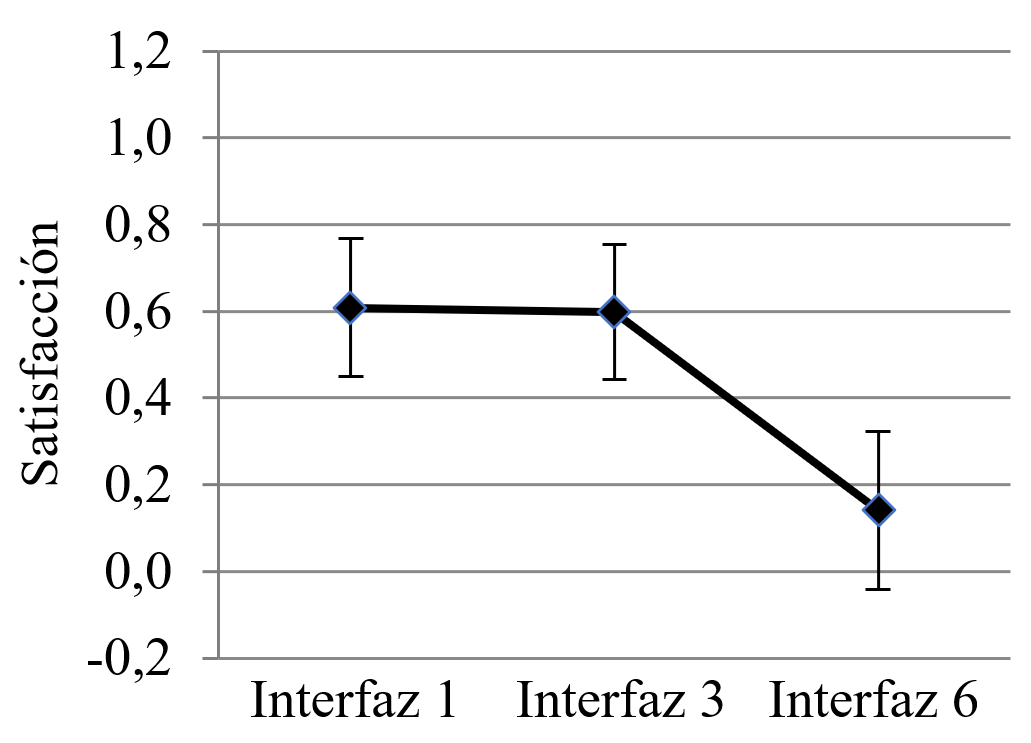
\includegraphics[width=\textwidth]{figures/3.9a.png}
    \caption{}
    \label{fig:3.9a}
  \end{subfigure}
  \hfill
  \begin{subfigure}[b]{0.45\textwidth}
    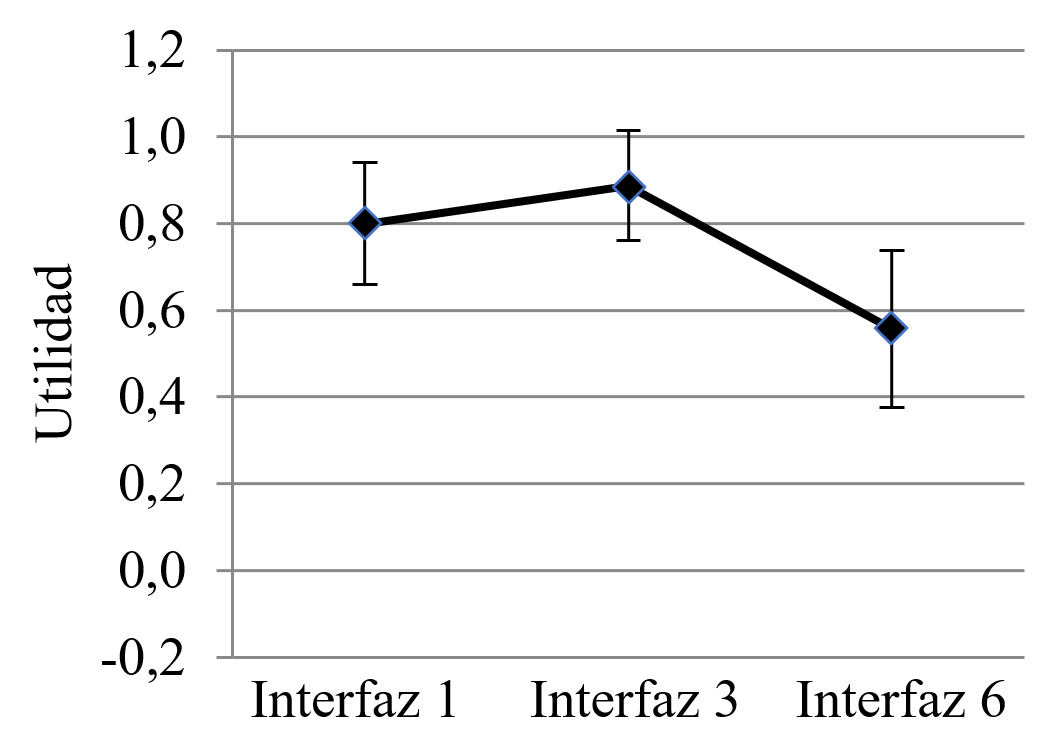
\includegraphics[width=\textwidth]{figures/3.9b.png}
    \caption{}
    \label{fig:3.9b}
  \end{subfigure}
  \begin{subfigure}[b]{0.45\textwidth}
    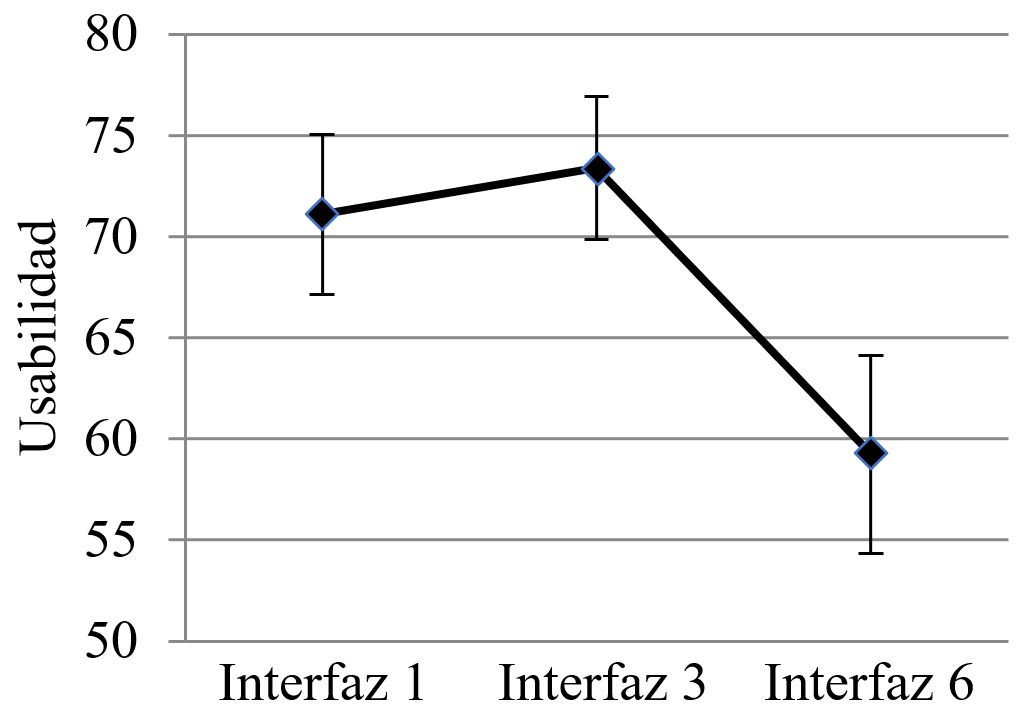
\includegraphics[width=\textwidth]{figures/3.9c.png}
    \caption{}
    \label{fig:3.9c}
  \end{subfigure}
  \caption{Media y error estándar de (a) Satisfacción (b) Utilidad (c) Usabilidad}
  \label{fig:3.9}
\end{figure}

\textbf{\emph{Medidas de esfuerzo mental}}

El esfuerzo mental fue evaluado mediante dos parámetros, uno subjetivo, representado por la Escala de Valoración del Esfuerzo Mental \gls{rsme}, y otro fisiológico utilizando el diámetro de la pupila. Los resultados relativos a la escala de esfuerzo mental mostraron diferencias significativas entre las interfaces 1 y 3 con la interfaz 6 (\emph{F} (2;44) = 5.57, \emph{p} = 0.007, $\eta^2$ = 0.2), siendo valorada esta última como más costosa de seguir que las anteriores. No se encontraron diferencias significanticas entre las interfaces 1 y 3. Los resultados pueden verse en la figura \ref{fig:3.10}.

\newpage
\begin{figure}[h]
    \centering
    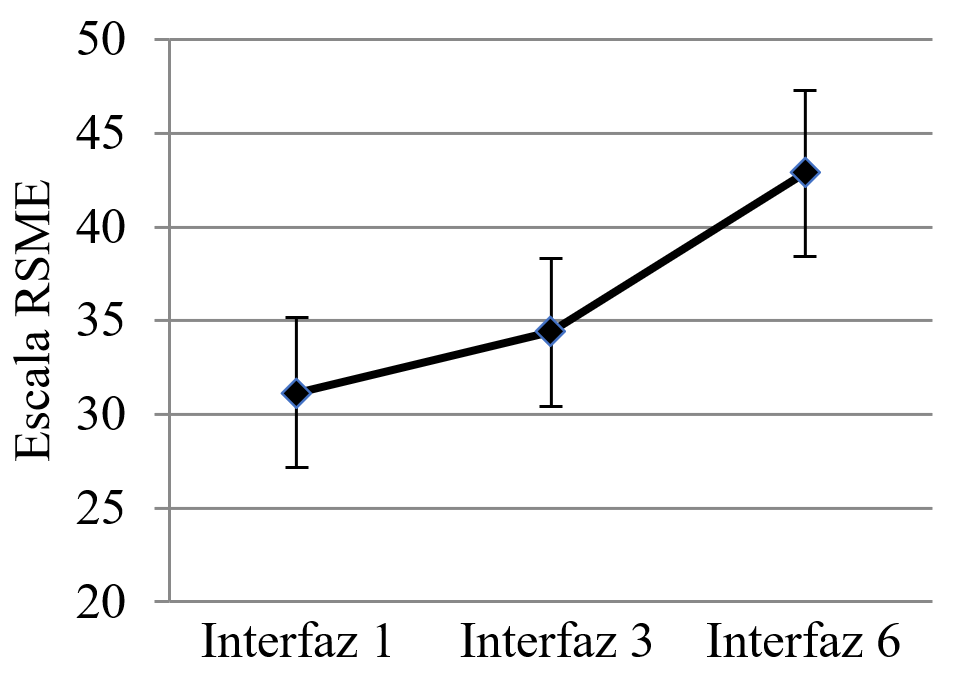
\includegraphics[width=7cm]
    {figures/3.10.png}
    \caption{ \label{fig:3.10} Media y error estándar de la Escala de Valoración de Esfuerzo Mental (\gls{rsme})}
\end{figure}

Para la variable fisiológica diámetro de la pupila, se encontraron diferencias estadísticamente significativas entre las situaciones sin interfaz o de línea base e interfaz activa (Figura \ref{fig:3.11}), con los valores de \emph{F} (3;57) = 19.68, \emph{p} < 0.001, $\eta^2$ = 0.51 para la pupila izquierda, y \emph{F} (3;57) = 17.31, \emph{p} < 0.001, $\eta^2$ = 0.48 para la pupila derecha. No obstante, no se encontraron diferencias entre las diferentes interfaces. Cabe añadir que el diámetro de la pupila no se vio afectado por los cambios lumínicos ya que las pruebas se realizaron en un laboratorio en condiciones estables. 

\begin{figure}[h]
  \centering
  \begin{subfigure}[b]{0.45\textwidth}
    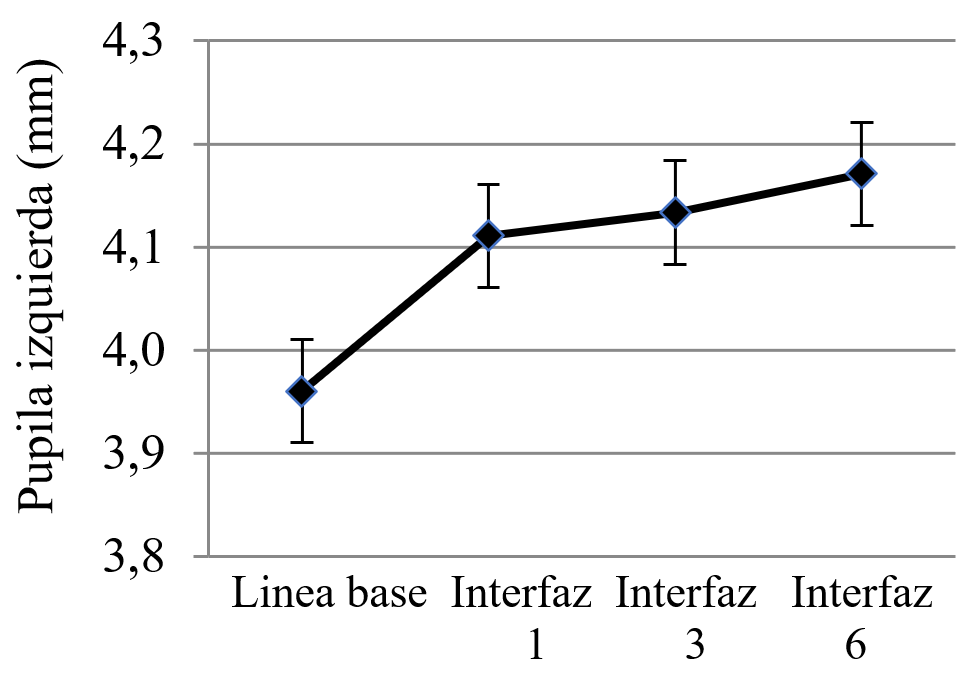
\includegraphics[width=\textwidth]{figures/3.11a.png}
    \caption{}
    \label{fig:3.11a}
  \end{subfigure}
  \hfill
  \begin{subfigure}[b]{0.45\textwidth}
    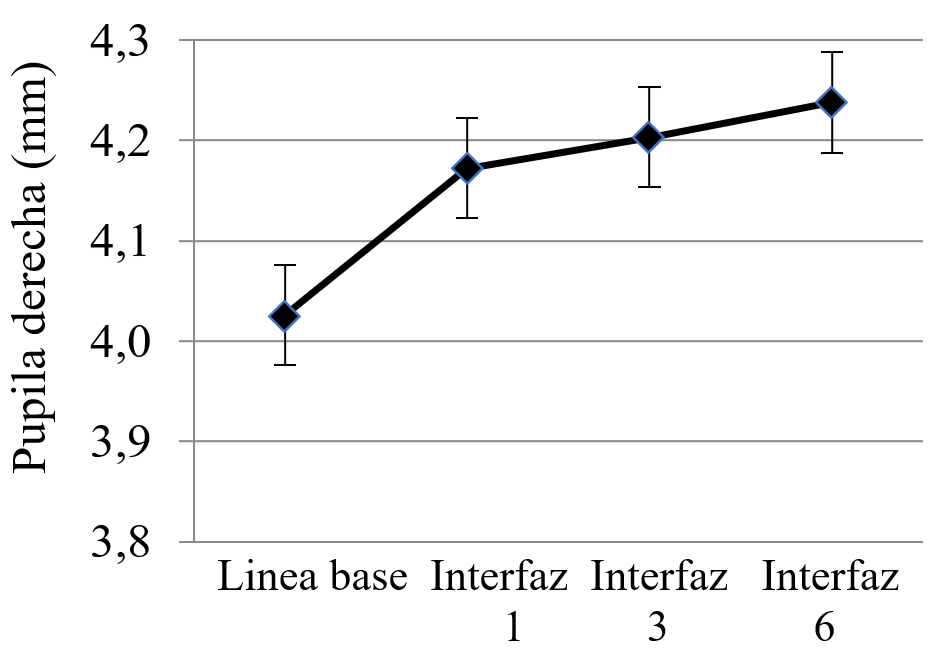
\includegraphics[width=\textwidth]{figures/3.11b.png}
    \caption{}
    \label{fig:3.11b}
  \end{subfigure}
  \caption{Media y error estándar del diámetro de las pupilas en la ausencia/presencia de las interfaces: (a) pupila izquierda, (b) pupila derecha}
  \label{fig:3.11}
\end{figure}

\textbf{\emph{Medidas oculares y seguimiento de la interfaz}}

En cuanto a otras medidas oculares utilizadas, como miradas, fijaciones y seguimiento de la interfaz en velocidad y giro de volante, no se encontraron diferencias estadísticamente significativas en función del diseño de la interfaz. En la tabla \ref{tab:3.8} se muestra un resumen del análisis de estas medidas durante las incorporaciones con los valores de la media, el error estándar y los resultados de la prueba \gls{anova}, cuyos resultados no son significativos.

\newpage
\begin{table}[h]
\centering
\begin{tabular}{rcc|cc|cc|cc}
\multirow{2}{*}{\textbf{Variable}} & \multicolumn{2}{c|}{\textbf{Interfaz 1}} & \multicolumn{2}{c|}{\textbf{Interfaz 3}} & \multicolumn{2}{c|}{\textbf{Interfaz 6}} & \multirow{2}{*}{\textbf{F}} & \multirow{2}{*}{\textbf{\emph{p}-valor}} \\ \cline{2-7}
                                   & \textit{M}         & \textit{SE}         & \textit{M}         & \textit{SE}         & \textit{M}         & \textit{SE}         &                             &                                   \\ \hline
TTM (s)*                           & 3.78               & 0.42                & 4.71               & 0.61                & 4.11               & 0.51                & 2.54                        & 0.09                              \\ \hline
Número de fijaciones               & 8.03               & 0.56                & 8.09               & 0.47                & 8.11               & 0.59                & 0.01                        & 0.98                              \\ \hline
Duración fijaciones (ms)           & 406                & 25                  & 468                & 40                  & 447                & 34                  & 2.04                        & 0.15                              \\ \hline
PTV*                               & 49\%               & 0.005               & 50\%               & 0.005               & 49\%               & 0.006               & 0.16                        & 0.85                              \\ \hline
PTVT*                              & 73\%               & 0.03                & 71\%               & 0.05                & 74\%               & 0.04                & 0.07                        & 0.80                              \\ \hline
\end{tabular}%
\caption{Media y error estándar de las medidas oculares y seguimiento de la interfaz}
\label{tab:3.8}
\end{table}

\textbf{\emph{Mapas de calor}}

Por último, se muestra a nivel visual un ejemplo de los mapas de calor de cada una de las interfaces ensayadas (Figura \ref{fig:3.12}). Relacionado con los resultados anteriores, se observa que los conductores dividen su atención hacia la interfaz, siendo este con el espejo retrovisor izquierdo y el carril central, uno de los tres puntos calientes característicos.

\begin{figure}[h]
  \centering
  \begin{subfigure}[b]{0.4\textwidth}
    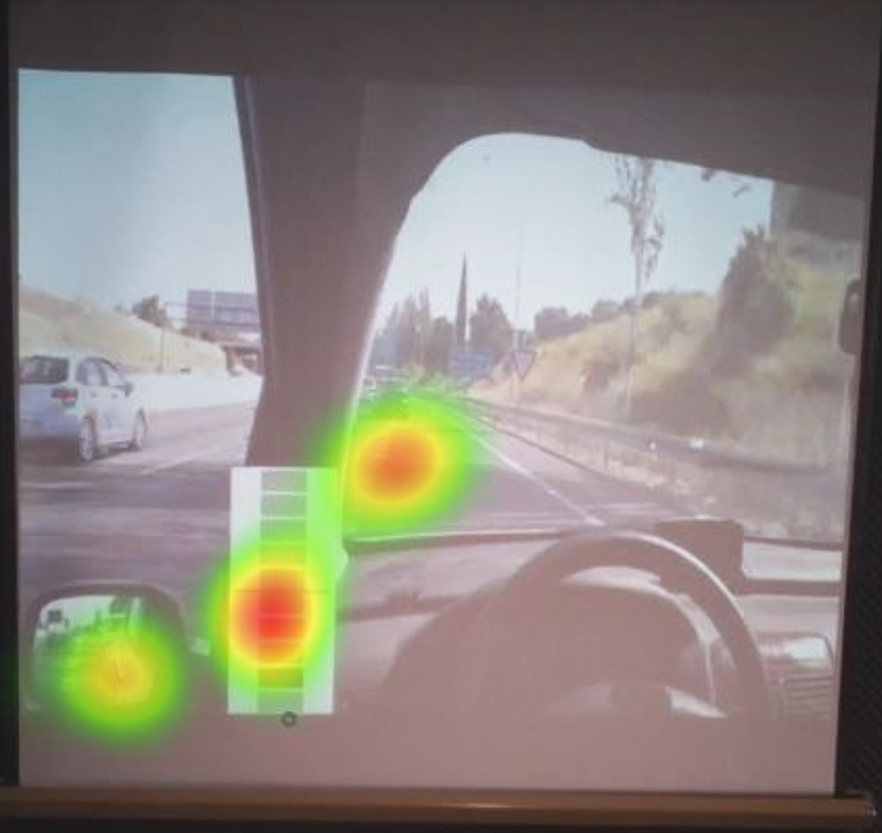
\includegraphics[width=\textwidth]{figures/3.12a.png}
    \caption{}
    \label{fig:3.12a}
  \end{subfigure}
  \hfill
  \begin{subfigure}[b]{0.4\textwidth}
    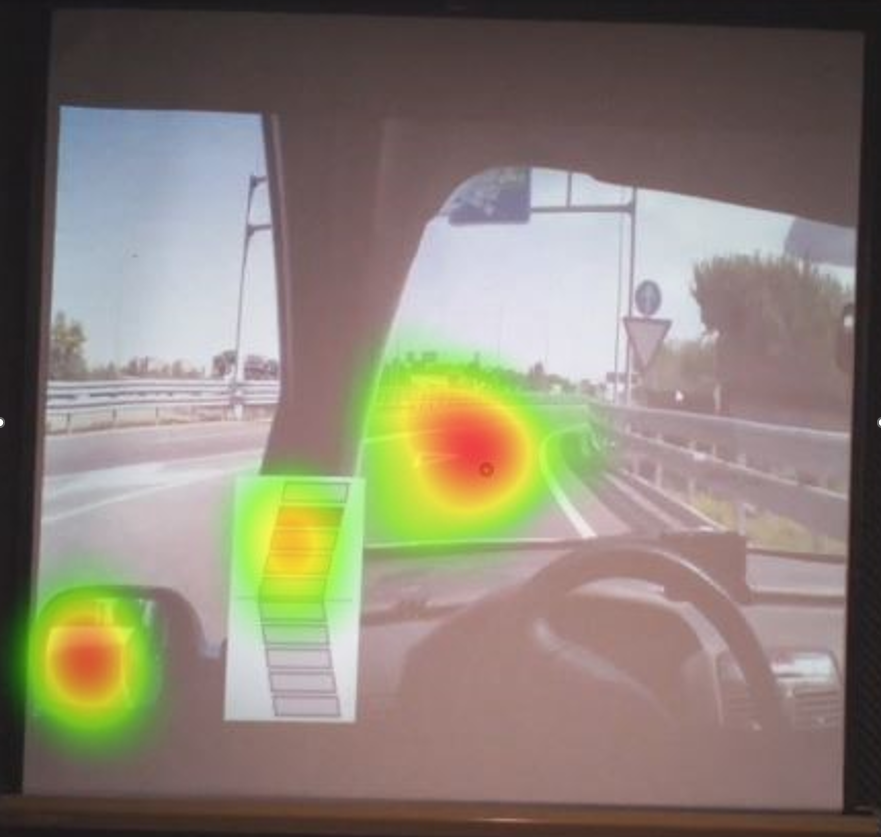
\includegraphics[width=\textwidth]{figures/3.12b.png}
    \caption{}
    \label{fig:3.12b}
  \end{subfigure}
  \begin{subfigure}[b]{0.4\textwidth}
    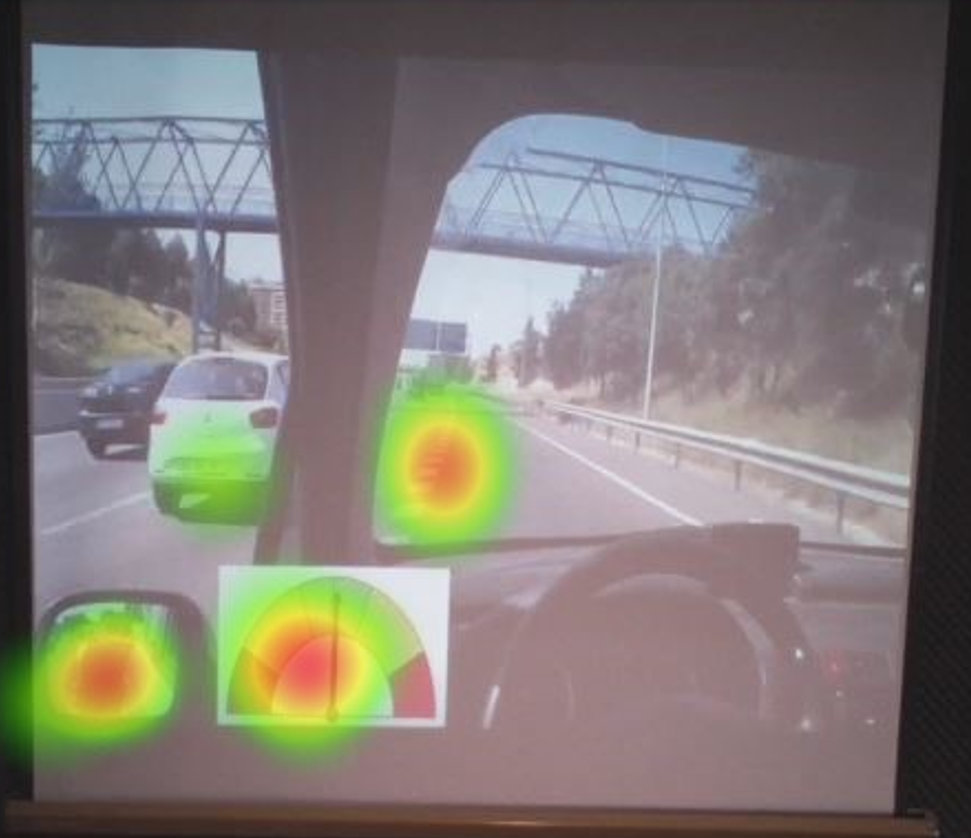
\includegraphics[width=\textwidth]{figures/3.12c.png}
    \caption{}
    \label{fig:3.12c}
  \end{subfigure}
  \caption{Mapas de calor para cada una de las interfaces durante una incorporación: (a) Interfaz 1, (b) Interfaz 3, (c) Interfaz 6}
  \label{fig:3.12}
\end{figure}

\subsubsection{3.1.3.4 Discusión}\label{3134}

Tres diseños de interfaz para un sistema de ayuda a la incorporación fueron evaluados en un simulador de conducción, atendiendo a encuestas sobre aceptación por parte del usuario y a variables atencionales del conductor. A nivel estadístico se encontraron diferencias en la aceptación por parte de los usuarios de las interfaces 1 o 3 frente a la interfaz 6, valorando las dos primeras como más satisfactorias, usables y útiles que la interfaz 6. Estas características son fundamentales cuando se desarrolla una nueva tecnología en los vehículos, ya que resulta improductivo invertir esfuerzos en el diseño y la construcción de un sistema si después no es utilizado o incluso se desactiva.

Considerando conjuntamente los resultados de las dos variables de esfuerzo mental, diámetro pupilar y \gls{rsme}, se puede concluir que seguir la interfaz 6 supone mayor esfuerzo que seguir las interfaces 1 y 3. Los resultados de \gls{rsme} mostraron diferencias significativas, y a pesar de que no se encontraron estas mismas diferencias para los diámetros pupilares entre interfaces, se puede percibir que sigue la misma tendencia que la escala \gls{rsme}. No obstante, sí se encontraron diferencias en la dilatación pupilar entre línea base y aparición de cualquier interfaz, numéricamente en torno al 3.5\%, mostrando de nuevo que el esfuerzo mental es mayor en la situación de incorporación. 

Otras medidas oculares mostraron similitud en los resultados recogidos entre interfaces, sin destacar ninguna diferencia significativa. Junto a los mapas de calor, se observa el correcto funcionamiento que han realizado los participantes durante el experimento, siendo el área de la interfaz junto a la del espejo izquierdo y el carril central, uno de los tres puntos calientes más mirados durante una incorporación. Tampoco se apreciaron efectos de orden ante la aparición de las interfaces, gracias a su aparición contrabalanceada.

Teniendo en cuenta todos los resultados, se descarta la interfaz 6 para la siguiente fase y se elige la interfaz 3 para implementarla en el sistema final, debido a que obtuvo resultados similares a la interfaz 1, pero aportando más información, como la dirección de la maniobra. En el siguiente estudio se realizan ensayos en conducción real con la interfaz propuesta, evaluando el funcionamiento del sistema mediante variables atencionales y encuestas de aceptación y carga mental.

\subsection{Validación de sistema de asistencia en incorporaciones en ensayos reales}\label{314}

Como se ha podido ver en fases anteriores, las variables atencionales del conductor proporcionan información sobre su estado ante diferentes eventos al igual que la aceptación de sistemas avanzados de ayuda o asistencia a la conducción (\gls{adas}). En el anterior estudio se propuso un sistema de ayuda a la incorporación mediante la generación de avisos basados en comunicaciones \gls{v2v}. En este estudio se implementa dicho sistema en conducción real, realizado ensayos bajo las mismas condiciones que en el simulador de conducción del subapartado \hyperref[313]{3.1.3.}. De la misma manera se registran los datos del seguimiento ocular, aceptabilidad y esfuerzo mental, añadiendo el cuestionario NASA-TLX sobre el índice de carga de la tarea. 

\subsubsection{3.1.4.1	Metodología}\label{3141}

Trece participantes, 2 de ellos mujeres, participaron en este estudio con edades comprendidas entre los 24 y los 43 años (\emph{M} = 31.53, \emph{SD} = 6.35). Su experiencia media al volante fue de 11.53 años (\emph{SD} = 6.59). 

Las pruebas de conducción real se realizaron en un tramo de la autovía M-45, situado en la zona sureste de Madrid, coincidiendo con tres zonas de incorporación señalizadas. Antes de realizar las pruebas reales, los conductores completaron la primera parte del cuestionario de carga de tareas de la NASA, en el que evaluaba subjetivamente la carga de trabajo de una tarea. 

Previo al inicio del ensayo los participantes eligieron la configuración de funcionamiento que les resultaba más intuitiva y se les pidió que condujeran de la forma más natural posible siguiendo las instrucciones de la interfaz. A continuación, se realizaron las pruebas con los vehículos instrumentados, el sistema de seguimiento ocular y el sistema de asistencia para ayudarles en las maniobras de incorporación.  Al finalizar la conducción realizaron la segunda parte del cuestionario de carga de tareas NASA junto a las encuestas de aceptación, usabilidad del sistema y esfuerzo mental sobre la interfaz. Finalmente, también respondieron a preguntas sobre información demográfica y si implementarían este sistema en su teléfono móvil si fuera gratuito. La duración media de cada sesión fue de aproximadamente quince minutos de conducción y cinco minutos más para responder a las escalas tras el ensayo. 

Las condiciones analizadas son las mismas que las descritas en el subapartado \hyperref[3121]{3.1.2.1.}, diferenciando los intervalos de incorporación del resto del ensayo (línea base) en base a la primera mirada al retrovisor. 

En esta última parte, el vehículo que realiza la incorporación fue instrumentado con el sistema de ayuda a la incorporación desarrollado en el subapartado \hyperref[313]{3.1.3}. El sistema fue soportado en un teléfono inteligente ubicado en la parte inferior del pilar A izquierdo del vehículo, tal y como se justifica en el subapartado \hyperref[3122]{3.1.2.2.} Las únicas entradas que necesita son los parámetros de posición y velocidad de ambos vehículos al final del carril, recogidos mediante un y enviados a través de módulos de comunicaciones desarrollados por INSIA y situados en cada uno de los vehículos (Figura \ref{fig:3.13}).

\begin{figure}[h]
    \centering
    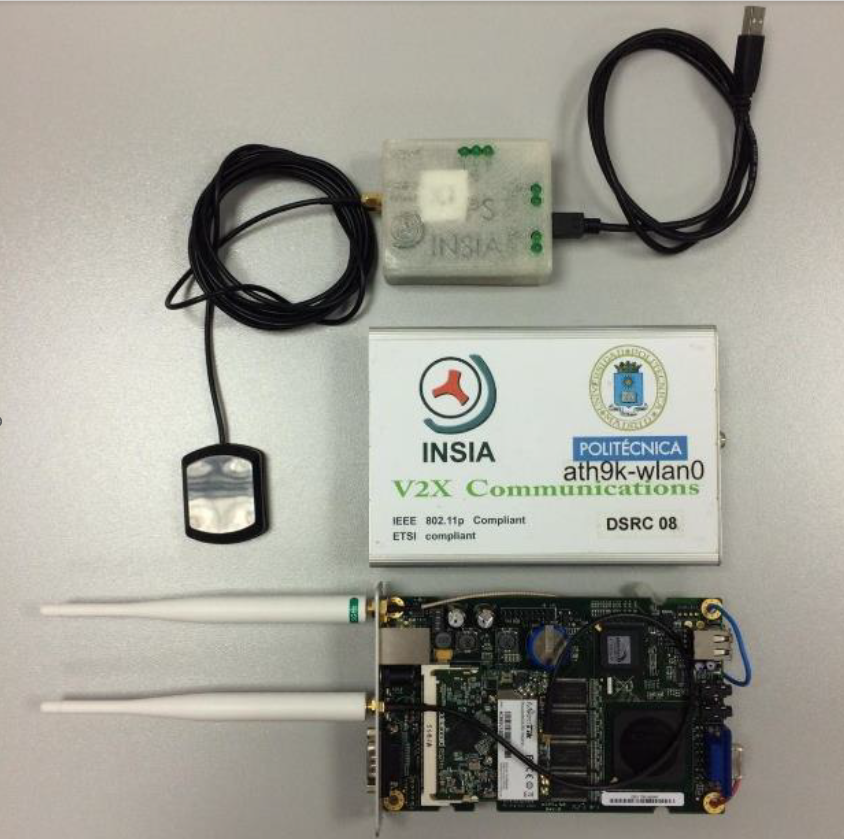
\includegraphics[width=8cm]
    {figures/3.13.png}
    \caption{ \label{fig:3.13} Módulo de comunicaciones y GNSS desarrollados por INSIA}
\end{figure}

Todos los vehículos implicados dispusieron de un módulo de comunicaciones Vehículo-a-vehículo (\gls{v2v}) acompañado de un Sistema Global de Navegación por Satélite (\gls{gnss}) de donde obtienen información sobre su posición y velocidad de ambos vehículos. Esta información llega desde los módulos vía WiFi a la aplicación de asistencia en incorporaciones, que genera avisos visuales al conductor (Figura \ref{fig:3.14}).

\newpage
\begin{figure}[h]
    \centering
    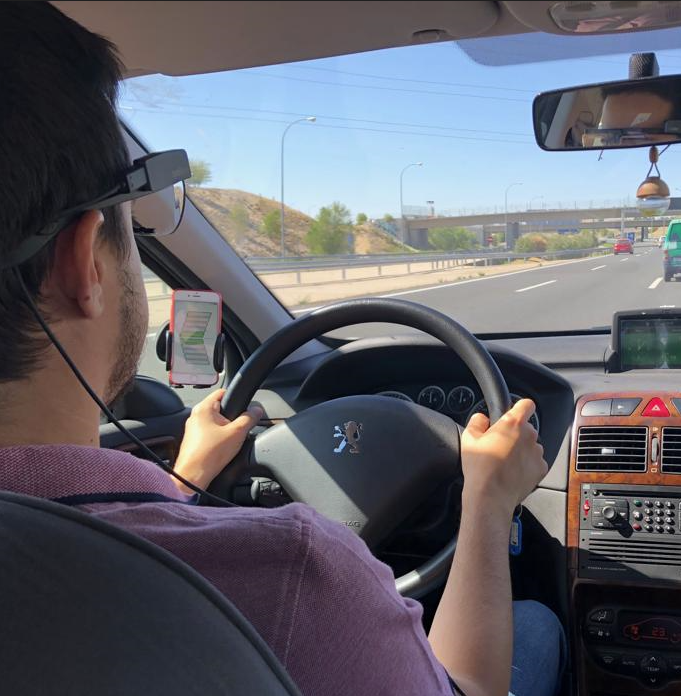
\includegraphics[width=8cm]
    {figures/3.14.png}
    \caption{ \label{fig:3.14} Aplicación de asistencia en incorporaciones en tráfico real}
\end{figure}

El uso de este sistema no condiciona la conducción en caso de ser ignorado y funciona solo como interfaz hombre-máquina, sin necesidad de ser manipulado durante la conducción. El análisis de la mirada también se realizó con el sistema de seguimiento ocular empleado en el subapartado \hyperref[3121]{3.1.2.1.}, al igual que el vehículo utilizado en la conducción. 

Para evaluar el funcionamiento del sistema de ayuda a la conducción se registraron las siguientes medidas al igual que en el subapartado \hyperref[313]{3.1.3.}: A) Aceptación del sistema (Satisfacción, Utilidad y Usabilidad); B) Esfuerzo mental (a través de dos medidas subjetivas, la Escala de Valoración del Esfuerzo Mental \gls{rsme} y el Índice de Carga de Tareas NASA-TLX; y de una medida fisiológica, la dilatación pupilar). 

Las encuestas utilizadas se encuentran descritas en el subapartado \hyperref[3132]{3.1.3.2.}, a excepción del cuestionario de carga de tareas que complementa al de esfuerzo mental. Este cuestionario es el Índice de Carga de Tareas de la Administración Nacional de la Aeronáutica y del Espacio (NASA-TLX) (\cite{hart}), el cual es ampliamente utilizado dado los sólidos argumentos alcanzados en investigación de factores humanos (\cite{pauzie}; \cite{rubio}). También se utiliza hoy en día para evaluar la carga de trabajo subjetiva y el esfuerzo cognitivo para una tarea proyectada en una \gls{hmi}, como en \textcite{pereira}, \textcite{matthews} y \textcite{papis}. Los cuestionarios de esfuerzo mental (\gls{rsme}) y carga de tareas, o de trabajo, (NASA-TLX) pueden resultar equivalentes por la terminología, pero evalúan desde diferentes enfoques la cognición frente a una tarea. El cuestionario de esfuerzo mental consiste en una escala unifactorial donde se puntúa cuanto esfuerzo requiere una tarea tras la realización de la misma. El cuestionario de carga de tareas evalúa las dimensiones de carga de trabajo, entre las que se encuentran demanda mental, demanda física, exigencia temporal, rendimiento, esfuerzo y frustración, analizando cada dimensión por pares antes y después de realizar la tarea. Algunas investigaciones utilizan ambas escalas para obtener un resultado más completo en sus estudios (\cite{sartang}; \cite{longo})

Los resultados de dilatación pupilar se analizaron mediante una prueba de rangos con signo de Wilcoxon para muestras pareadas con el fin de verificar si existen diferencias estadísticamente significativas. Por último, se calculó el coeficiente de correlación de Pearson o \emph{r} con objeto de hallar relaciones entre las variables obtenidas de este estudio. Los análisis estadísticos se realizaron con el software estadístico SPSS v26.

\subsubsection{3.1.4.2 Resultados}\label{3142}
\textbf{\emph{Medidas de satisfacción, utilidad y usabilidad}}

Los resultados de aceptación del sistema de ayuda en conducción real se resumen a continuación. En la tabla \ref{tab:3.9} se muestra la media y el error estándar junto a su correspondiente escala, observándose que las puntuaciones recogidas se encuentran por encima del valor medio. 


\begin{table}[h]
\centering
\begin{tabular}{rclcc}
               & \multicolumn{2}{c}{\textbf{Satisfacción}} & \textbf{Utilidad} & \textbf{Usabilidad} \\ \hline
Media          & \multicolumn{2}{c}{0.3269}                & 0.1385            & 65.193              \\ \hline
Error estándar & \multicolumn{2}{c}{0.1843}                & 0.1623            & 4.7910              \\ \hline
Escala         & \multicolumn{2}{c}{-2 ; +2}               & -2 ; +2           & 0 ; 100             \\ \hline
\end{tabular}
\caption{Media, error estándar y escala de satisfacción, utilidad y usabilidad}
\label{tab:3.9}
\end{table}

A pesar de que los resultados son meramente descriptivos, se puede considerar que los usuarios valoran positivamente el sistema de asistencia.

\textbf{\emph{Medidas de esfuerzo mental}}

El esfuerzo mental que pueda suponer atender al sistema durante la maniobra de incorporación se ha analizado mediante la Escala de Valoración del Esfuerzo Mental \gls{rsme} y el Índice de Carga de Tareas NASA-TLX. En la tabla \ref{tab:3.10} se exponen los resultados de la media y el error estándar junto a sus escalas.

\begin{table}[h]
\centering
\begin{tabular}{rllc}
               & \multicolumn{2}{l}\textbf{\gls{rsme}} & \textbf{NASA-TLX} \\ \hline
Media          & \multicolumn{2}{l}{37.6923}       & 0.1385            \\ \hline
Error estándar & \multicolumn{2}{l}{4.6207}        & 0.1623            \\ \hline
Escala         & \multicolumn{2}{l}{0 ; 150}       & 0 ; 100           \\ \hline
\end{tabular}
\caption{Media, error estándar y escala de \gls{rsme} y NASA-TLX}
\label{tab:3.10}
\end{table}

Se advierte que ambas variables se encuentran por debajo del valor medio, siendo la carga mayor que el esfuerzo. Dado que no es posible comparar con otros sistemas, la puntuación más fiable en este campo sería NASA-TLX, ya que además se basa en las puntuaciones antes y después del uso del sistema. 

En cuanto a las medidas de seguimiento ocular, no se encontraron diferencias estadísticamente significativas en el tamaño de la pupila durante las incorporaciones en función de la aparición del sistema de asistencia, ni para la pupila del ojo izquierdo ni para la del derecho, \emph{Z} = -0.594, \emph{p} = 0.552 y \emph{Z} = -0.664, \emph{p} = 0.507, respectivamente. Estos resultados apoyan la hipótesis de que en ambas situaciones la carga es la misma y que el uso del sistema de asistencia no implica un sobreesfuerzo para los conductores, probablemente debido al estrés propio que requiere la situación de incorporación (Tabla \ref{tab:3.11}).

\newpage
\begin{table}[]
\centering
\begin{tabular}{rcccc}
               & \multicolumn{2}{c}{\textbf{\begin{tabular}[c]{@{}c@{}}Diámetro de   pupila\\  izquierda\end{tabular}}} & \multicolumn{2}{c}{\textbf{\begin{tabular}[c]{@{}c@{}}Diámetro de   pupila\\  derecha\end{tabular}}} \\ \cline{2-5} 
\textit{}      & \textit{Con \gls{adas}}                                  & \textit{Sin \gls{adas}}                                 & \textit{Con \gls{adas}}                                 & \textit{Sin \gls{adas}}                                \\ \hline
Media          & 2.2754                                             & 2.2780                                            & 2.2915                                            & 2.3070                                           \\ \hline
Error estándar & 0.045                                              & 0.055                                             & 0.045                                             & 0.054                                            \\ \hline
\end{tabular}
\caption{Media y error estándar del diámetro de la pupila izquierda y derecha durante la incorporación con y sin el sistema de asistencia (\gls{adas})}
\label{tab:3.11}
\end{table}

\textbf{\emph{Correlaciones entre variables}}

Las posibles relaciones lineales entre las variables obtenidas de todos los participantes fueron estudiadas mediante el coeficiente de correlación de Pearson (\emph{r}). Se realizó un análisis entre todas las variables adquiridas durante el ensayo de conducción real, encontrando correlaciones estadísticamente significativas en algunas de ellas (Tabla \ref{tab:3.12}). 


\begin{table}[h]
\centering
\begin{tabular}{rcccc}
                                  & \textbf{Usabilidad}                                                  & \textbf{\gls{rsme}}                                                     & \textbf{NASA-TLX}                                               & \textbf{Utilidad}                                                     \\ \hline
Satisfacción                      & \begin{tabular}[c]{@{}c@{}}\emph{r} = 0.84\\ \emph{p} \textless 0.001\end{tabular} & \begin{tabular}[c]{@{}c@{}}\emph{r} = -0.56\\    \emph{p} = 0.048\end{tabular}  & \cellcolor[HTML]{C9C9C9}\textit{}                               & \cellcolor[HTML]{C9C9C9}\textit{}                            \\ \hline
Diámetro de la   pupila           & \cellcolor[HTML]{C9C9C9}                                             & \begin{tabular}[c]{@{}c@{}}\emph{r} = 0.66\\    \emph{p} =   0.014\end{tabular} & \cellcolor[HTML]{C9C9C9}                                        & \cellcolor[HTML]{C9C9C9}                                     \\ \hline
Número de   fijaciones            & \cellcolor[HTML]{C9C9C9}                                             & \cellcolor[HTML]{C9C9C9}                                          & \begin{tabular}[c]{@{}c@{}}\emph{r} = 0.57\\    \emph{p} = 0.042\end{tabular} & \cellcolor[HTML]{C9C9C9}                                     \\ \hline
Número de   miradas a la interfaz & \cellcolor[HTML]{C9C9C9}                                             & \cellcolor[HTML]{C9C9C9}                                          & \cellcolor[HTML]{C9C9C9}                                        & \begin{tabular}[c]{@{}c@{}}\emph{r} = 0.67\\ \emph{p} = 0.013\end{tabular} \\ \hline
\end{tabular}
\caption{Correlaciones significativas entre medidas (p\textless{}0.05)}
\label{tab:3.12}
\end{table}


\subsubsection{3.1.4.3	Discusión}\label{3143}

El sistema de asistencia a la incorporación presentado ha sido validado en ensayos reales, obteniendo resultados satisfactorios en cuanto a ejecución y operatividad. Los resultados muestran que los conductores valoraron positivamente el sistema, dado que las puntuaciones de aceptación se situaron por encima del valor medio. La comparativa de maniobra de incorporación con y sin \gls{adas} revela que no hubo diferencias significativas en el diámetro de la pupila de ambas situaciones, difiriendo los valores menos de un 0.5\%, por lo que se puede deducir que existe una carga mental debida a la maniobra, la cual queda reflejada en las variables \gls{rsme} y NASA-TLX, pero que no es vinculante con la aparición de la interfaz. 

Por último, se encontraron relaciones interesantes entre las variables estudiadas. La satisfacción que tiene un conductor sobre un sistema tiene una fuerte relación con su percepción de usable, al igual que también con su sensación de exigencia en términos cognitivos. En una interfaz valorada como útil también aumentó el número de miradas a la misma, implicando un mayor seguimiento visual del sistema. Sin embargo, este seguimiento se vio afectado negativamente ante la relación de carga de trabajo, obtenida de NASA-TLX, y número de fijaciones. Una mirada compuesta de muchas fijaciones indica que el conductor debe examinar detenidamente el área de la interfaz para poder obtener la suficiente información antes de dirigir su atención a otra parte, lo cual es peligroso ante un entorno tan cambiante. Por último, resalta la asociación entre las medidas de esfuerzo mental, dilatación pupilar y las puntuaciones \gls{rsme}, validando esta relación como herramienta para futuros ensayos en tráfico real.

La implementación del sistema \gls{hmi} se realiza en un smartphone, debido a la flexibilidad que proporciona la plataforma en el proceso de diseño e integración, sin embargo, se pretende que en futuras versiones la interfaz este implementada en los controles del vehículo o en la estructura del mismo. Esta configuración mejoraría las condiciones visuales del puesto de conducción al no considerar el sistema como un dispositivo independiente que pudiera distraer al conductor.

\section{Adelantamientos en conducción parcialmente automatizada}\label{32}

La acción de adelantar es frecuentemente utilizada por los conductores, tanto para llegar a un destino como para adquirir unas condiciones deseables de circulación. Sin embargo, según el informe de la \gls{nhtsa} (\cite{sen}), el cambio de carril es considerada una maniobra de riesgo debido a la alta probabilidad de accidente en caso de distracción. En \textcite{shawky}, un 57.2\% de los encuestados expusieron que la distracción durante un cambio de carril fue el principal motivo de realizar maniobras repentinas e inseguras, de los cuales 36\% manifestaron que la distracción fue debida a mantener conversaciones con los ocupantes del vehículo y 21.2\% a usar el teléfono móvil. También es interesante el dato que arroja sobre miradas a los espejos laterales y miradas a las ventanas en busca de puntos ciegos previo a un cambio de carril, donde los conductores que inspeccionaron dichas áreas tuvieron menos posibilidades de verse involucrados en colisiones con otros vehículos, 4.61 y 3.85 veces respectivamente. 

En el progreso hacia la automatización de vehículos se han realizado grandes avances en el desarrollo de \gls{adas}, procurando maniobras más seguras y reduciendo el riesgo de accidentes. El cambio de carril junto al seguimiento del vehículo, se consideran las principales acciones que fundamentan los modelos de conducción actuales y los algoritmos de toma de decisiones. Los \gls{adas} orientados al seguimiento de un vehículo han obtenido resultados favorables tanto a nivel tecnológico como social, siendo muy común su integración en los vehículos actuales. Ejemplo de ello son los sistemas de control de crucero adaptativo (\gls{acc}), y de frenada de emergencia (\gls{aeb}). Sin embargo, no ocurre lo mismo para los sistemas de cambio de carril automático, ya que, debido a diversas razones como la naturaleza de la maniobra, el marco legal de cada país o los diferentes perfiles de conducción, son escasas sus apariciones en vehículos comerciales dada su falta de madurez. No obstante, y a pesar de que el proceso de cambio de carril no es totalmente automático, sistemas como el asistente de mantenimiento de carril (\gls{ldw}), y detección de ángulo muerto (\gls{bsd}) ayudan a que su ejecución se produzca con seguridad y control.

Actualmente la maniobra de adelantamiento es totalmente manual en los vehículos con automatización nivel 2 y puede empezarse a ver en algunos modelos nivel 3, cuya función solo se activa ante determinadas circunstancias ideales de seguridad, como carreteras en perfectas condiciones, líneas de carril bien pintadas, condiciones climáticas estables, etc.

En este capítulo se estudian las variables atencionales del conductor a través de la maniobra de cambio de carril en un vehículo parcialmente autónomo nivel 2. Los datos analizados fueron adquiridos en 2018 en el Instituto Nacional Sueco de Investigación de Carreteras y Transportes (en sueco: \gls{vti}). El propósito de estos ensayos fue analizar, mediante un sistema de seguimiento visual, la influencia de la experiencia de los conductores en un vehículo modelo Volvo con el sistema \gls{pa2}. Las condiciones se dieron en conducción manual y parcialmente automatizada mientras se realizaba una tarea secundaria en una vía de alta capacidad en tráfico real. Los resultados obtenidos durante toda la conducción reflejaron que el nivel 2 no aligeraba cognitivamente al conductor en la realización de tareas adicionales, ni siquiera con experiencia previa en el sistema de automatización (\cite{solismarcos}). Este hecho fue debido a la constante monitorización del testigo del modo autónomo ubicado en el panel de mandos por parte del conductor. En las grabaciones se puede observar que, en determinadas ocasiones, el sistema se desconectaba sin más advertencia que la visual, posiblemente porque no consideraría seguro el entorno.

Gracias a esta base de datos adquirida en dichos ensayos y a la cual se permitió el acceso para su explotación, este estudio se ha centrado en la maniobra de adelantamiento para conductores con experiencia, siendo interesante la capa de información del comportamiento visual del conductor a la tarea secundaria y la posibilidad de automatización parcial. Los estudios realizados se han dividido en tres partes:

\begin{itemize}
    \item \hyperref[3231]{Distribución visual durante un adelantamiento}
    \item \hyperref[3232]{Análisis de la secuencia visual durante un adelantamiento}
    \item \hyperref[3233]{Miradas a la tarea secundaria según fases de un adelantamiento}
\end{itemize}

En primer lugar, se analiza la distribución de miradas en el entorno del cambio de carril, analizando cómo cambia el peso de cada objeto mirado a lo largo de la maniobra. De igual manera, se estudia la secuencia de miradas a los objetos, obteniendo las relaciones más frecuentes que permitan definan futuros patrones en la conducción. Por último, las miradas a la tarea en las fases del adelantamiento determinan qué periodos considera el conductor menos demandantes para poder dirigir su atención a la tarea, procurando una buena gestión atencional. La base de datos ha sido cedida por el \gls{vti} para los análisis propuestos.

\subsection{Definición de un adelantamiento y sus fases}\label{321}

La maniobra de cambio de carril ha sido segmentada principalmente en dos etapas: periodo de anticipación al cambio de carril y estabilización en carril contiguo. El criterio de inicio del periodo de anticipación fue determinado en base a observaciones comunes a todas las maniobras realizadas. El principal indicador de adelantamiento fue la preparación visual del conductor mediante una sucesión de miradas consecutivas al espejo retrovisor izquierdo, ocasionalmente combinadas con miradas al espejo retrovisor interior. Por otro lado, se estudió el intervalo temporal que dedicó el conductor a la preparación de la maniobra, el cual tuvo una relación lineal directa con las miradas realizadas (Figura \ref{fig:3.15}). 

\begin{figure}[h]
    \centering
    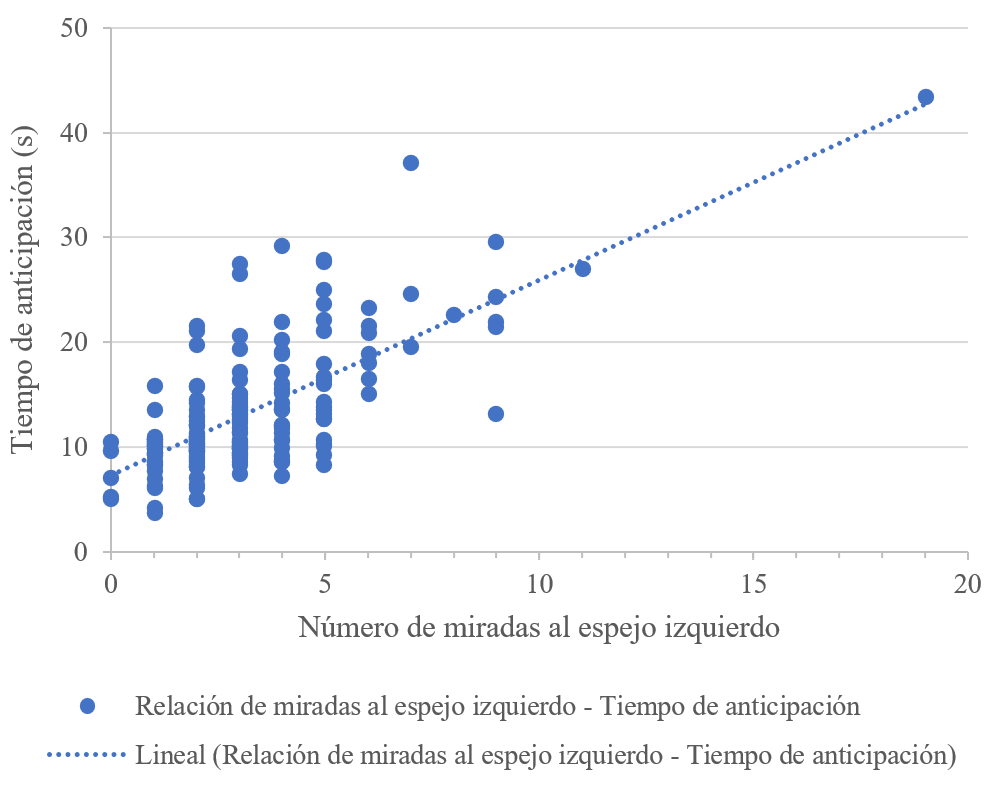
\includegraphics[width=12.5cm]
    {figures/3.15.png}
    \caption{ \label{fig:3.15} Relación de miradas al espejo retrovisor izquierdo con el tiempo de anticipación }
\end{figure}

En las siguientes gráficas se muestra en detalle los resultados obtenidos de toda la muestra para ambas variables (Figura \ref{fig:3.16a} y \ref{fig:3.16b}).

\begin{figure}[h]
  \centering
  \begin{subfigure}[b]{0.45\textwidth}
    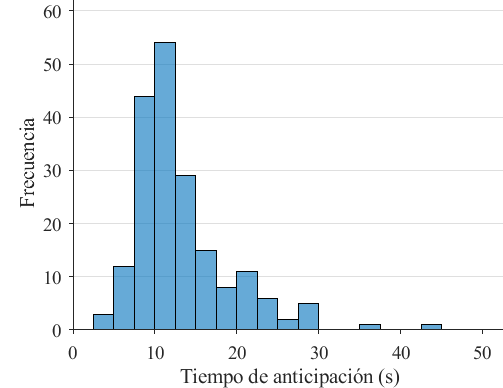
\includegraphics[width=\textwidth]{figures/3.16a.png}
    \caption{}
    \label{fig:3.16a}
  \end{subfigure}
  \hfill
  \begin{subfigure}[b]{0.45\textwidth}
    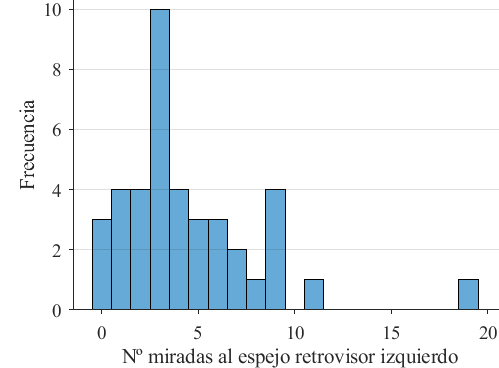
\includegraphics[width=\textwidth]{figures/3.16b.png}
    \caption{}
    \label{fig:3.16b}
  \end{subfigure}
  \caption{(a) Frecuencia del tiempo de anticipación, (b) Frecuencia del número de miradas al espejo retrovisor izquierdo}
  \label{fig:3.16}
\end{figure}

En la figura \ref{fig:3.16a}, se observa que el tiempo de anticipación se produjo en intervalos de entre 4 y 30 segundos antes de cruzar la línea central de la carretera, realizándose a los 10 segundos en la mayoría de los adelantamientos. El número mínimo de miradas para este fenómeno se produjese se determinó en 3, como se observa de forma destacable en la figura \ref{fig:3.16b}. Además, también se pudo advertir que algunos conductores desconectaron la tarea antes de realizar la maniobra, lo que refuerza aún más la indicación de adelantar al vehículo objetivo.
En el análisis de miradas a la tarea se han subdividido dichas etapas, obteniendo cuatro fases diferenciadas en la realización de un adelantamiento: circulación en el carril derecho, \gls{acd}, circulación en el carril izquierdo y \gls{aci} (Figura \ref{fig:3.17}).

\begin{figure}[h]
    \centering
    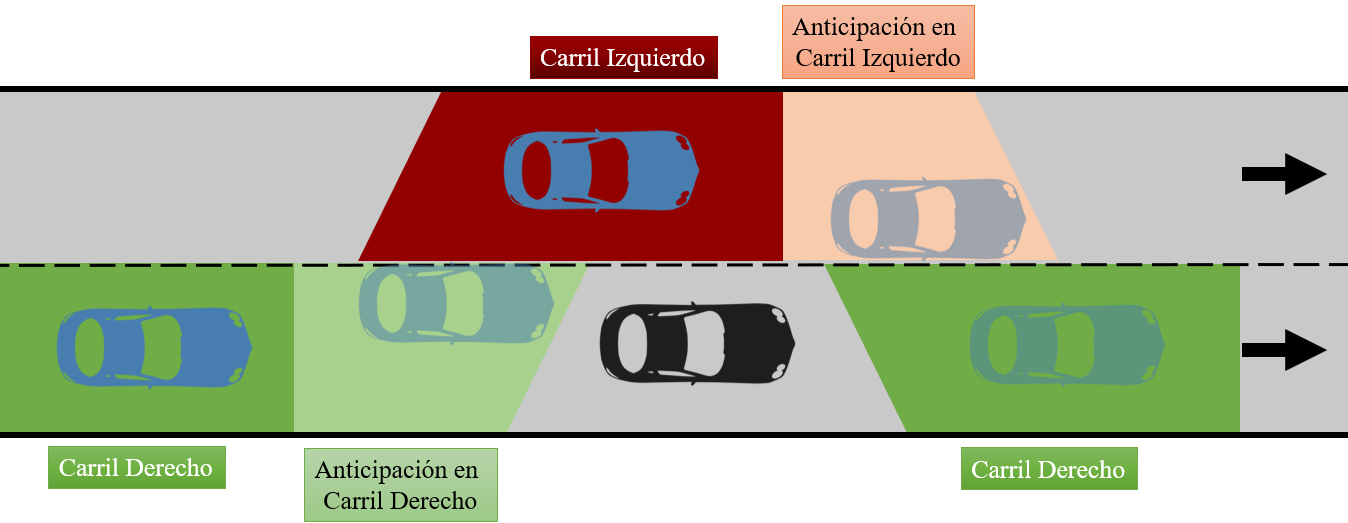
\includegraphics[width=14cm]
    {figures/3.17.png}
    \caption{ \label{fig:3.17} Segmentación de las fases en un cambio de carril}
\end{figure}

\subsection{Metodología }\label{322}

Los participantes del estudio fueron un total de 23 conductores, divididos entre 9 conductores con experiencia previa en el vehículo utilizado y 12 sin experiencia, de los cuales 2 de ellos fueron mujeres. Para el objeto de este estudio solo se han tenido en cuenta los participantes experimentados, siendo todos ellos hombres, elegidos por ser conductores habituales de un vehículo modelo Volvo equipado con el sistema \gls{pa2} de asistencia al pilotaje. También fue requisito el uso de este sistema al menos 3 veces por semana durante un mes. Todos los conductores fueron recompensados con 500SEK (aproximadamente 50€) por su participación en el experimento. La edad de los participantes fue de 47 años (\emph{SD} = 10.74) y la experiencia en conducción de media 29 años (\emph{SD} = 10.74). Dada la naturaleza de este ensayo, es destacable señalar que el protocolo experimental ha respetado el Código Ético de la Asociación Estadounidense de Psicología (\gls{apa}) y fue aprobado por el Comité Regional de Revisión Ética en Linköping, Suecia (DNR: 2016/411- 31).

Los ensayos fueron realizados en una autopista de la ciudad sueca de Linköping en un tramo de 7.5 km de ida y los mismos para la vuelta, siendo su límite de velocidad 110 km/h. Se detectaron un total de 110 adelantamientos, 60 en manual y 50 en modo autónomo, realizando un promedio de 3.05 maniobras por conductor en cada condición y una desviación estándar de 1.47. Durante la conducción, los participantes debían realizar una tarea visuomotora soportada en una tablet ubicada a la derecha del volante. La tarea consistía en una matriz 4 x 4 de flechas apuntado hacia abajo, donde el participante debía señalar si existía algún elemento que apuntase hacia arriba lo más rápido posible mediante los botones \emph{SI} y \emph{NO}, primando siempre la seguridad. Una nueva matriz aparecía cuando el conductor daba una respuesta o después de los 5 segundos si no se registraba nada en el sistema. La tarea disponía de dos modos de funcionamiento: tarea forzosa, la cual demandaba respuestas durante todo el proceso de conducción, y tarea pausable, donde los conductores podían desconectar la tarea mediante un botón sin afectar a su rendimiento, encendiéndola de nuevo en el momento que lo considerasen. En base la puntuación obtenida al finalizar el ensayo, los conductores fueron incentivados lúdicamente con el fin de evitar el exceso de desconexión de la tarea. Para la condición de conducción parcialmente automatizada, se pidió a los conductores que utilizasen el sistema \gls{pa2} en la medida de lo posible, desactivándolo cuando lo considerase necesario. 

El diseño del experimento fue 2 x 2 x 2, con tres variables intrasujeto correspondientes a los niveles de automatización (manuela y autónomo), la pausabilidad de la tarea y la fase del adelantamiento. Todos los participantes realizaron las cuatro condiciones experimentales de manera contrabalanceada para evitar efectos de orden, como la fatiga o el aprendizaje. Las condiciones se resumen en: A) Conducción automatizada + tarea adicional forzosa, B) Conducción automatizada + tarea adicional pausable, C) Conducción manual + tarea adicional forzosa, y D) Conducción manual + tarea adicional pausable. Para las cuatro condiciones solo se eligieron los tramos de adelantamiento que se produjeron dentro de la autopista, y en el último subapartado del estudio, se segmentaron las cuatro fases del adelantamiento definidas anteriormente.

El vehículo utilizado fue un Volvo S90 del 2017 equipado con la segunda versión del sistema de asistencia a la conducción (\gls{pa2}). Dicho sistema combina el funcionamiento de control de crucero adaptativo (\gls{acc}) y el asistente de mantenimiento de carril (\gls{lka}), cuya activación se realiza mediante de los mandos del volante como se indica en la figura \ref{fig:3.18}. El testigo situado bajo el velocímetro indica su estado, presentándose en color verde si el sistema estaba activado en su totalidad o en color gris cuando tenía dificultades para detectar las marcas de carril, funcionando únicamente el \gls{acc}. El vehículo dispone de sensores en el volante que permiten al conductor retirar las manos durante un máximo de 15 segundos cuando el sistema está activado. Si tras ese intervalo no detectase al conductor, el sistema se desconectaría automáticamente por seguridad, indicándolo mediante el testigo visual. 

\newpage
\begin{figure}[h]
    \centering
    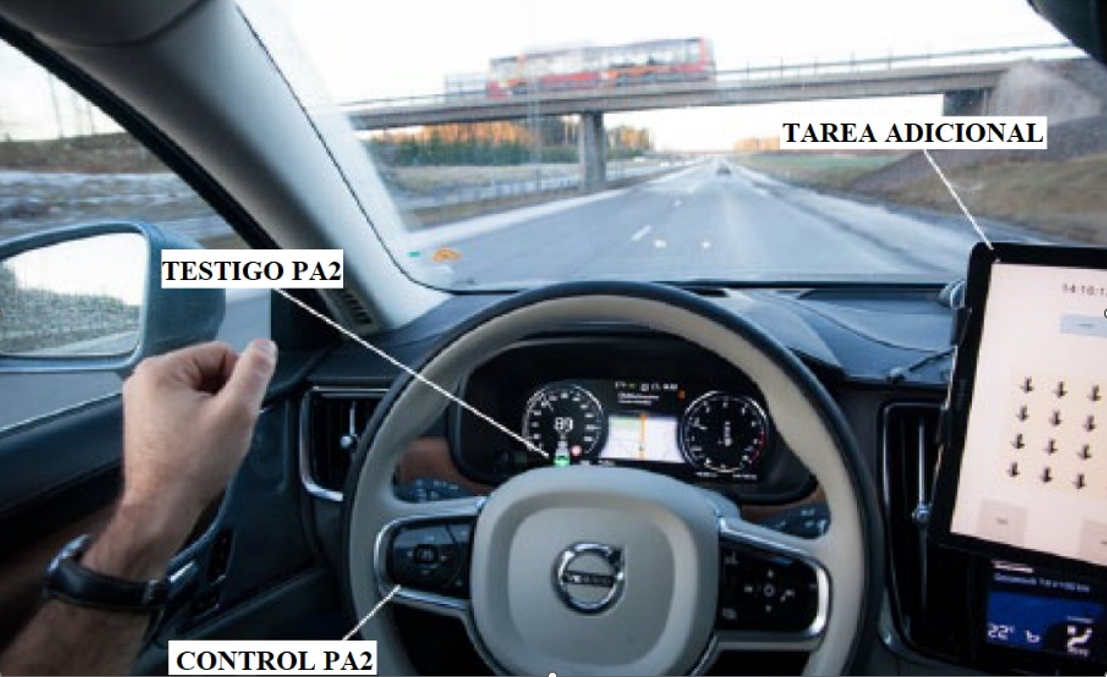
\includegraphics[width=11cm]
    {figures/3.18.png}
    \caption{ \label{fig:3.18} Vista interior vehículo, tarea adicional, símbolo activación del sistema \gls{pa2} (original en \textcite{solismarcos})}
\end{figure}

La adquisición de datos se realizó mediante un par de cámaras que grababan la vista frontal del vehículo y al estado de activación del sistema \gls{pa2}, marca Video VBox Pro. Se utilizó un sistema de posicionamiento global interno (\gls{gps}) para registrar la velocidad, posición y hora, con una frecuencia 10 Hz, y un sistema de seguimiento ocular, marca SMI Eye Tracking Glasses 2.0, para registrar el estado atencional del conductor. Este sistema consiste en unas gafas sensorizadas equipadas con sensores infrarrojos que permiten detectar el comportamiento de la mirada mediante la técnica pupila oscura mencionada anteriormente. Las gafas también disponen de una cámara orientada hacia la escena frontal, que permite la grabación de la mirada del conductor en la carretera. Las variables obtenidas para su procesamiento se observan en la tabla \ref{tab:3.13}.

\begin{table}[h]
\centering
\begin{tabular}{rll}
\textbf{Variables}     & \textbf{Descripción}           & \textbf{Unidades}           \\ \hline
Duración               & Duración del evento observado  & Milisegundos                \\ \hline
Codificación           & Condición del ensayo realizado &                             \\ \hline
Evento                 & Ítem observado                 &                             \\ \hline
Tipo de evento         & Inicio y fin de cada evento    &                             \\ \hline
Video                  & Grabación del ensayo           & 1280 x 960 píxeles a 25 fps \\ \hline
Frecuencia de muestreo &                                & 60 Hz                       \\ \hline
Precisión              &                                & 0.5°                       \\ \hline
\end{tabular}
\caption{Variables del sistema de seguimiento visual SMI Eye Tracking Glasses 2.0}
\label{tab:3.13}
\end{table}

Para el tratamiento de los datos se realizó una fusión del sistema de seguimiento ocular con los videos capturados por las cámaras mediante el software BeGaze Version 3.7. Los eventos fueron codificados manualmente con el software Observer XT Version 13, al igual que las áreas de interés, las cuales fueron panel de mandos, frente, espejo interior, espejo izquierdo, espejo derecho, tarea y otros. El área frente se define como las miradas al carril por el que circula y otros incluye las miradas a los carriles adyacentes, señales y otras zonas del interior del vehículo. Posteriormente se superpusieron los datos adquiridos por la tarea adicional con el resto de los datos para su análisis global.

En cuanto a pruebas estadísticas, se ha aplicado un modelo lineal mixto generalizado utilizando el software Jamovi 2.2.5 con objetivo de analizar la dependencia entre las variables adquiridas por el sistema de seguimiento visual. El ajuste de las comparaciones se realizó mediante el procedimiento de Holm.

\subsection{Resultados}\label{323}

En las condiciones donde la tarea fue pausable, se analizó la probabilidad de que el conductor interrumpiera la tarea durante una maniobra de adelantamiento. Los resultados muestran que solamente el 8.3\% de los conductores pausó la aplicación en conducción parcialmente automatizada, y un 6.2\% en conducción manual, para las condiciones donde la tarea era pausable, B y D respectivamente.

En base a estos resultados, los estudios se han reducido a las condiciones de manual y parcialmente automatizada, ya que no se poseen demasiados datos para la condición de pausabilidad ni se considera que pueda existir ningún efecto significativo, rediseñando el diseño del experimento a 2 x 2 con dos variables intrasujeto y eliminando las incorporaciones donde la tarea estuvo pausada.

\textbf{\emph{Distribución visual durante un adelantamiento}}\label{3231}

La relación de miradas a las diferentes áreas definidas anteriormente ha sido evaluada porcentualmente, observando la variación de pesos a cada objeto a lo largo de la maniobra. Las áreas se definen en panel de mandos, frente, espejo interior, espejo izquierdo, espejo derecho, tarea y otro. La ventana temporal comienza 10 segundos antes del cruce de la línea central, como se explicó anteriormente en el apartado \hyperref[321]{3.2.1.} Definición de un adelantamiento y sus fases, y termina 5 segundos después, a modo informativo sobre la dirección de la mirada tras el cambio de carril. El instante 0 corresponde al evento donde se definió el cruce de la línea que separa los carriles. Las siguientes gráficas representan un adelantamiento de derecha a izquierda (Figura \ref{fig:3.19}) en conducción manual y conducción parcialmente automatizada. 

\begin{figure}[h]
    \centering
    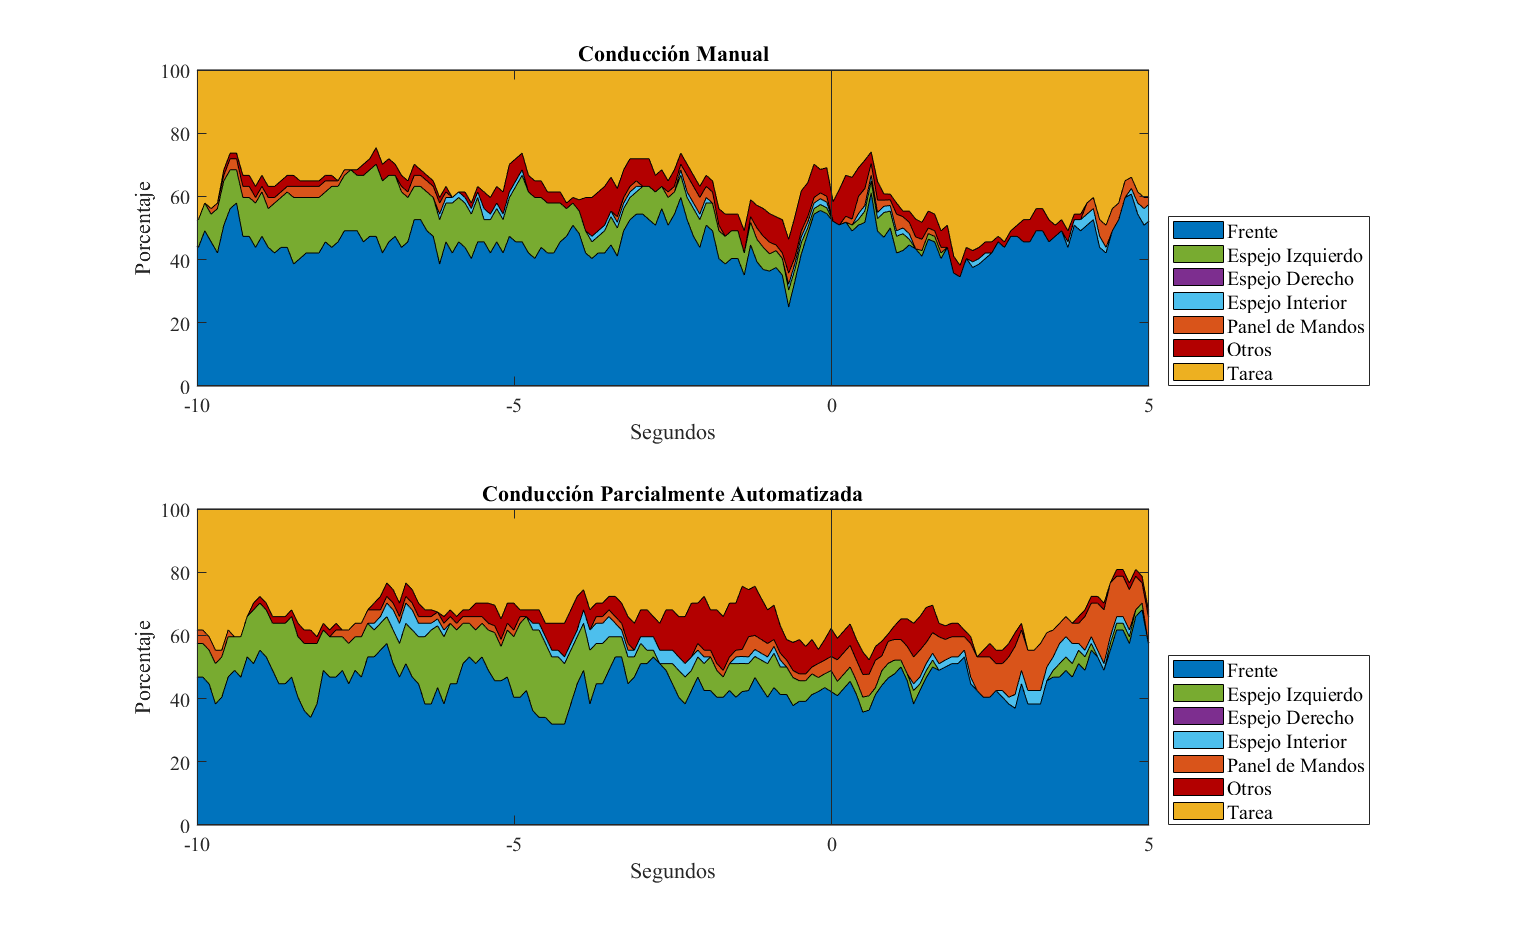
\includegraphics[width=16cm]
    {figures/3.19.png}
    \caption{ \label{fig:3.19} Distribución visual de las miradas durante un adelantamiento en conducción manual y parcialmente automatizada}
\end{figure}

\textbf{\emph{Análisis de la secuencia visual durante un adelantamiento}}\label{3232}

El conjunto de áreas observadas durante un cambio de carril ha sido estudiado analizando la secuencia visual realizada por el conductor. Los resultados se presentan en forma de tabla de probabilidad por parejas contraponiendo las zonas a estudiar para conducción manual y parcialmente automatizada, donde la serie se inicia con el parámetro situado a la izquierda (Entrada) y termina con el parámetro superior (Salida) (Tablas \ref{tab:3.14} y \ref{tab:3.15}). El porcentaje refleja la probabilidad de que se realice una inspección visual desde una entrada y termine en una determinada salida, respecto a la totalidad de las parejas de miradas.

% Please add the following required packages to your document preamble:
% \usepackage[table,xcdraw]{xcolor}
% If you use beamer only pass "xcolor=table" option, i.e. \documentclass[xcolor=table]{beamer}
\begin{table}[h]
\centering
\begin{tabular}{|lccccccc|}
\hline
\multicolumn{8}{|c|}{\textbf{Porcentajes en conducción manual}}                                        \\ \hline
\multicolumn{1}{|l|}{\textit{\begin{tabular}[c]{@{}l@{}}\diagbox[width=9em]{Salida}{Entrada}\end{tabular}}} & \multicolumn{1}{c|}{\textit{\begin{tabular}[c]{@{}c@{}}Panel de \\ mandos\end{tabular}}} & \multicolumn{1}{c|}{\textit{Frente}}               & \multicolumn{1}{c|}{\textit{\begin{tabular}[c]{@{}c@{}}Espejo \\ interior\end{tabular}}} & \multicolumn{1}{c|}{\textit{\begin{tabular}[c]{@{}c@{}}Espejo \\ izquierdo\end{tabular}}} & \multicolumn{1}{c|}{\textit{\begin{tabular}[c]{@{}c@{}}Espejo \\ derecho\end{tabular}}} & \multicolumn{1}{c|}{\textit{Tarea}}                & \textit{Otros}               \\ \hline
\multicolumn{1}{|l|}{\textit{Panel de mandos}}                                                & \multicolumn{1}{c|}{\cellcolor[HTML]{C9C9C9}}                                            & \multicolumn{1}{c|}{\cellcolor[HTML]{EFF5FC}2.62}  & \multicolumn{1}{c|}{\cellcolor[HTML]{FCFCFF}0}                                           & \multicolumn{1}{c|}{\cellcolor[HTML]{FCFCFF}0}                                            & \multicolumn{1}{c|}{\cellcolor[HTML]{FCFCFF}0}                                          & \multicolumn{1}{c|}{\cellcolor[HTML]{FBFCFF}0.26}  & \cellcolor[HTML]{FCFCFF}0.09 \\ \hline
\multicolumn{1}{|l|}{\textit{Frente}}                                                         & \multicolumn{1}{c|}{\cellcolor[HTML]{EFF4FC}2.71}                                        & \multicolumn{1}{c|}{\cellcolor[HTML]{C9C9C9}}      & \multicolumn{1}{c|}{\cellcolor[HTML]{F3F7FD}1.92}                                        & \multicolumn{1}{c|}{\cellcolor[HTML]{D6E5F5}7.70}                                         & \multicolumn{1}{c|}{\cellcolor[HTML]{FAFBFF}0.44}                                       & \multicolumn{1}{c|}{\cellcolor[HTML]{5F9ED7}31.50} & \cellcolor[HTML]{EFF4FC}2.71 \\ \hline
\multicolumn{1}{|l|}{\textit{Espejo interior}}                                                & \multicolumn{1}{c|}{\cellcolor[HTML]{FCFCFF}0}                                           & \multicolumn{1}{c|}{\cellcolor[HTML]{F6F8FE}1.40}  & \multicolumn{1}{c|}{\cellcolor[HTML]{C9C9C9}}                                            & \multicolumn{1}{c|}{\cellcolor[HTML]{FCFCFF}0}                                            & \multicolumn{1}{c|}{\cellcolor[HTML]{FCFCFF}0.09}                                       & \multicolumn{1}{c|}{\cellcolor[HTML]{F9FAFF}0.70}  & \cellcolor[HTML]{FCFCFF}0    \\ \hline
\multicolumn{1}{|l|}{\textit{Espejo izquierdo}}                                               & \multicolumn{1}{c|}{\cellcolor[HTML]{FCFCFF}0}                                           & \multicolumn{1}{c|}{\cellcolor[HTML]{D5E5F5}7.87}  & \multicolumn{1}{c|}{\cellcolor[HTML]{FCFCFF}0}                                           & \multicolumn{1}{c|}{\cellcolor[HTML]{C9C9C9}}                                             & \multicolumn{1}{c|}{\cellcolor[HTML]{FCFCFF}0}                                          & \multicolumn{1}{c|}{\cellcolor[HTML]{F7F9FE}1.14}  & \cellcolor[HTML]{FCFCFF}0.17 \\ \hline
\multicolumn{1}{|l|}{\textit{Espejo derecho}}                                                 & \multicolumn{1}{c|}{\cellcolor[HTML]{FCFCFF}0}                                           & \multicolumn{1}{c|}{\cellcolor[HTML]{FCFCFF}0.17}  & \multicolumn{1}{c|}{\cellcolor[HTML]{FCFCFF}0}                                           & \multicolumn{1}{c|}{\cellcolor[HTML]{FCFCFF}0}                                            & \multicolumn{1}{c|}{\cellcolor[HTML]{C9C9C9}}                                           & \multicolumn{1}{c|}{\cellcolor[HTML]{FCFCFF}0.17}  & \cellcolor[HTML]{FCFCFF}0    \\ \hline
\multicolumn{1}{|l|}{\textit{Tarea}}                                                          & \multicolumn{1}{c|}{\cellcolor[HTML]{FCFCFF}0.17}                                        & \multicolumn{1}{c|}{\cellcolor[HTML]{5B9BD5}32.28} & \multicolumn{1}{c|}{\cellcolor[HTML]{FCFCFF}0.17}                                        & \multicolumn{1}{c|}{\cellcolor[HTML]{FBFCFF}0.26}                                         & \multicolumn{1}{c|}{\cellcolor[HTML]{FCFCFF}0}                                          & \multicolumn{1}{c|}{\cellcolor[HTML]{C9C9C9}}      & \cellcolor[HTML]{F7F9FE}1.14 \\ \hline
\multicolumn{1}{|l|}{\textit{Otros}}                                                          & \multicolumn{1}{c|}{\cellcolor[HTML]{FCFCFF}0.09}                                        & \multicolumn{1}{c|}{\cellcolor[HTML]{F0F5FC}2.54}  & \multicolumn{1}{c|}{\cellcolor[HTML]{FCFCFF}0.09}                                        & \multicolumn{1}{c|}{\cellcolor[HTML]{FBFCFF}0.26}                                         & \multicolumn{1}{c|}{\cellcolor[HTML]{FCFCFF}0}                                          & \multicolumn{1}{c|}{\cellcolor[HTML]{F6F9FE}1.31}  & \cellcolor[HTML]{C9C9C9}     \\ \hline
\end{tabular}
\caption{Secuencias visuales durante un adelantamiento en conducción manual}
\label{tab:3.14}
\end{table}

% Please add the following required packages to your document preamble:
% \usepackage[table,xcdraw]{xcolor}
% If you use beamer only pass "xcolor=table" option, i.e. \documentclass[xcolor=table]{beamer}
\begin{table}[h]
\centering
\begin{tabular}{|llllllll|}
\hline
\multicolumn{8}{|c|}{\textbf{Porcentajes en conducción parcialmente automatizada}} 
\\ \hline
\multicolumn{1}{|l|}{\textit{\begin{tabular}[c]{@{}l@{}}\diagbox[width=9em]{Salida}{Entrada}\end{tabular}}} & \multicolumn{1}{c|}{\textit{\begin{tabular}[c]{@{}c@{}}Panel de \\ mandos\end{tabular}}} & \multicolumn{1}{c|}{\textit{Frente}}               & \multicolumn{1}{c|}{\textit{\begin{tabular}[c]{@{}c@{}}Espejo \\ interior\end{tabular}}} & \multicolumn{1}{c|}{\textit{\begin{tabular}[c]{@{}c@{}}Espejo \\ izquierdo\end{tabular}}} & \multicolumn{1}{c|}{\textit{\begin{tabular}[c]{@{}c@{}}Espejo \\ derecho\end{tabular}}} & \multicolumn{1}{c|}{\textit{Tarea}}                & \multicolumn{1}{c|}{\textit{Otros}} \\ \hline
\multicolumn{1}{|l|}{\textit{Panel de mandos}}                                                & \multicolumn{1}{l|}{\cellcolor[HTML]{C9C9C9}}                                            & \multicolumn{1}{l|}{\cellcolor[HTML]{D9E7F6}5.95}  & \multicolumn{1}{l|}{\cellcolor[HTML]{FCFCFF}0}                                           & \multicolumn{1}{l|}{\cellcolor[HTML]{FCFCFF}0}                                            & \multicolumn{1}{l|}{\cellcolor[HTML]{FCFCFF}0}                                          & \multicolumn{1}{l|}{\cellcolor[HTML]{F7F9FE}0.86}  & \cellcolor[HTML]{FBFCFF}0.22        \\ \hline
\multicolumn{1}{|l|}{\textit{Frente}}                                                         & \multicolumn{1}{l|}{\cellcolor[HTML]{D7E6F6}6.16}                                        & \multicolumn{1}{l|}{\cellcolor[HTML]{C9C9C9}}      & \multicolumn{1}{l|}{\cellcolor[HTML]{F4F7FD}1.41}                                        & \multicolumn{1}{l|}{\cellcolor[HTML]{C4DAF1}9.41}                                         & \multicolumn{1}{l|}{\cellcolor[HTML]{FCFCFF}0}                                          & \multicolumn{1}{l|}{\cellcolor[HTML]{619FD7}25.73} & \cellcolor[HTML]{EAF1FB}3.14        \\ \hline
\multicolumn{1}{|l|}{\textit{Espejo interior}}                                                & \multicolumn{1}{l|}{\cellcolor[HTML]{FCFCFF}0}                                           & \multicolumn{1}{l|}{\cellcolor[HTML]{F5F8FE}1.19}  & \multicolumn{1}{l|}{\cellcolor[HTML]{C9C9C9}}                                            & \multicolumn{1}{l|}{\cellcolor[HTML]{FCFCFF}0}                                            & \multicolumn{1}{l|}{\cellcolor[HTML]{FBFCFF}0.22}                                       & \multicolumn{1}{l|}{\cellcolor[HTML]{FBFBFF}0.32}  & \cellcolor[HTML]{FCFCFF}0           \\ \hline
\multicolumn{1}{|l|}{\textit{Espejo izquierdo}}                                               & \multicolumn{1}{l|}{\cellcolor[HTML]{FCFCFF}0}                                           & \multicolumn{1}{l|}{\cellcolor[HTML]{C1D9F0}9.84}  & \multicolumn{1}{l|}{\cellcolor[HTML]{FCFCFF}0}                                           & \multicolumn{1}{l|}{\cellcolor[HTML]{C9C9C9}}                                             & \multicolumn{1}{l|}{\cellcolor[HTML]{FCFCFF}0}                                          & \multicolumn{1}{l|}{\cellcolor[HTML]{F9FAFE}0.65}  & \cellcolor[HTML]{FBFCFF}0.22        \\ \hline
\multicolumn{1}{|l|}{\textit{Espejo derecho}}                                                 & \multicolumn{1}{l|}{\cellcolor[HTML]{FCFCFF}0}                                           & \multicolumn{1}{l|}{\cellcolor[HTML]{FCFCFF}0.11}  & \multicolumn{1}{l|}{\cellcolor[HTML]{FCFCFF}0}                                           & \multicolumn{1}{l|}{\cellcolor[HTML]{FCFCFF}0}                                            & \multicolumn{1}{l|}{\cellcolor[HTML]{C9C9C9}}                                           & \multicolumn{1}{l|}{\cellcolor[HTML]{FCFCFF}0.11}  & \cellcolor[HTML]{FCFCFF}0           \\ \hline
\multicolumn{1}{|l|}{\textit{Tarea}}                                                          & \multicolumn{1}{l|}{\cellcolor[HTML]{F9FAFE}0.65}                                        & \multicolumn{1}{l|}{\cellcolor[HTML]{5B9BD5}26.70} & \multicolumn{1}{l|}{\cellcolor[HTML]{FBFBFF}0.32}                                        & \multicolumn{1}{l|}{\cellcolor[HTML]{FBFBFF}0.32}                                         & \multicolumn{1}{l|}{\cellcolor[HTML]{FCFCFF}0}                                          & \multicolumn{1}{l|}{\cellcolor[HTML]{C9C9C9}}      & \cellcolor[HTML]{F4F7FD}1.41        \\ \hline
\multicolumn{1}{|l|}{\textit{Otros}}                                                          & \multicolumn{1}{l|}{\cellcolor[HTML]{FBFBFF}0.32}                                        & \multicolumn{1}{l|}{\cellcolor[HTML]{ECF3FB}2.70}  & \multicolumn{1}{l|}{\cellcolor[HTML]{FBFCFF}0.22}                                        & \multicolumn{1}{l|}{\cellcolor[HTML]{FBFCFF}0.22}                                         & \multicolumn{1}{l|}{\cellcolor[HTML]{FCFCFF}0}                                          & \multicolumn{1}{l|}{\cellcolor[HTML]{F3F7FD}1.62}  & \cellcolor[HTML]{C9C9C9}            \\ \hline
\end{tabular}
\caption{Secuencias visuales durante un adelantamiento en conducción parcialmente automatizada}
\label{tab:3.15}
\end{table}

Los colores representan las relaciones más frecuentes y la intensidad los valores más altos. Los valores obtenidos representan de manera numérica los resultados del apartado anterior \emph{Distribución visual durante un adelantamiento}. 

\textbf{\emph{Miradas a la tarea secundaria según fases de un adelantamiento}}\label{3233}

Las relaciones de los parámetros obtenidos del sistema de seguimiento visual, duración media de miradas y número de miradas por segundo a la tarea, han sido estudiadas mediante un modelo lineal mixto generalizado. Dado que el nivel de pausabilidad de la tarea no se ha considerado relevante, debido a la escasa cantidad de datos, el modelo queda reducido a los niveles de automatización y fase. Se observaron efectos principales en la duración media de miradas a la tarea en la condición automatización (\emph{F} (1;109) = 7.85, \emph{p} = 0.006) y en fase (\emph{F} (1;109) = 11.94, \emph{p} < 0.001), al igual que para el número de miradas por segundo a la tarea en la condición automatización (\emph{F} (1;107) = 10.78, \emph{p} = 0.001) y en fase (\emph{F} (1;107) = 4.19, \emph{p} = 0.008).
Estos efectos pueden verse en la figura \ref{fig:3.20} y figura \ref{fig:3.21} para ambas variables, a través de la representación de las medias en cada modo de automatización por fases.  

\begin{figure}[h]
    \centering
    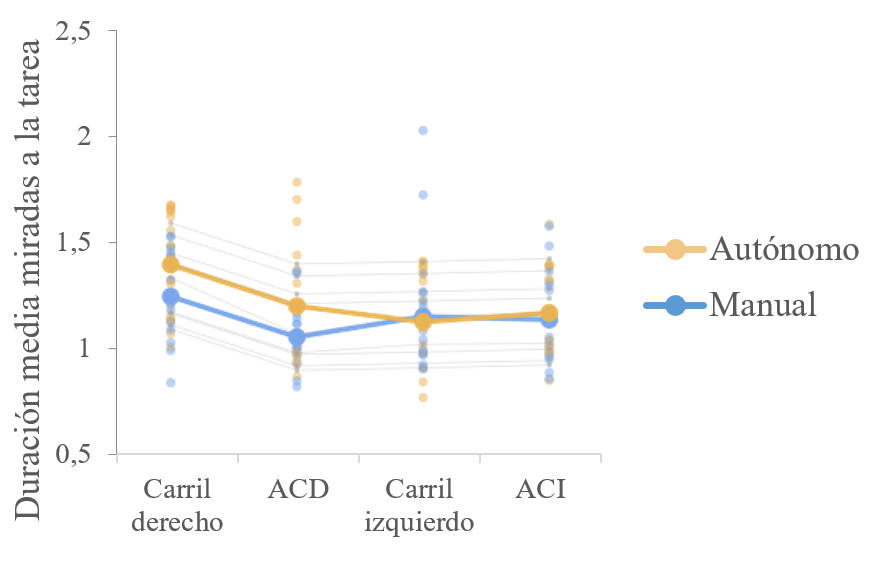
\includegraphics[width=10.5cm]
    {figures/3.20.png}
    \caption{ \label{fig:3.20} Efectos en duración media de miradas a la tarea en cada modo de automatización por fases del adelantamiento}
\end{figure}

\begin{figure}[h]
    \centering
    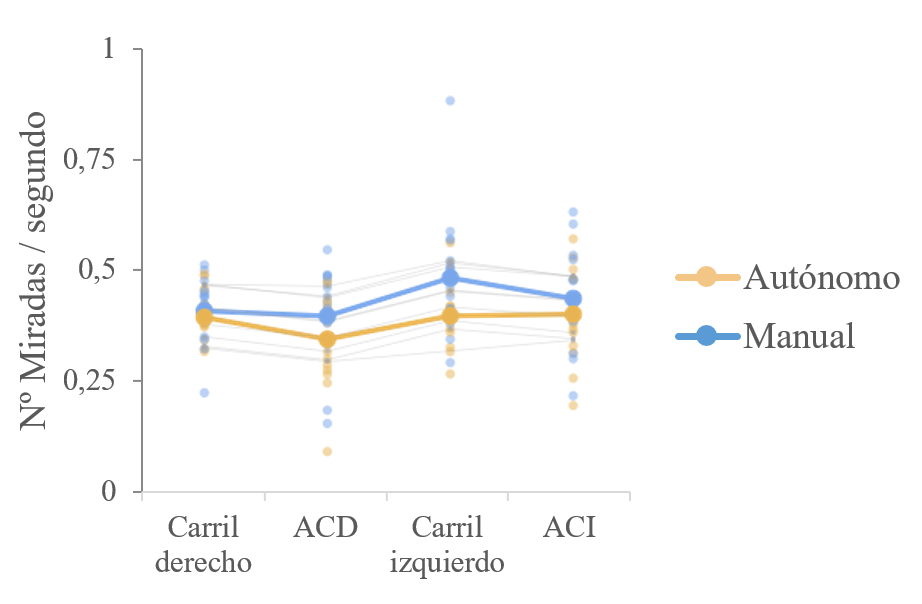
\includegraphics[width=10.5cm]
    {figures/3.21.png}
    \caption{ \label{fig:3.21} Efectos en número de miradas por segundo a la tarea en cada modo de automatización por fases del adelantamiento}
\end{figure}

Se puede apreciar que en duración media existe un efecto en carril derecho y en \gls{acd}, destacando que todos los datos los valores para autónomo son mayores que manual. Por el contrario, el número de fijaciones fueron mayores en manual que en autónomo, donde el efecto aparece en la zona de carril izquierdo. Los efectos aleatorios se muestran al fondo en línea fina. 

Para valorar si el efecto es significativo, en la tabla \ref{tab:3.16} se recogen los valores p de cada zona en función del nivel de automatización.

\begin{table}[h]
\centering
\begin{tabular}{rccl}
\textbf{}                                                                      & \multicolumn{3}{c}{\textbf{Valor \emph{p} entre modos de automatización}}                                                                                                                     \\ \hline
\textbf{Fases del adelantamiento}                                              & \begin{tabular}[c]{@{}c@{}}Duración media \\ miradas a la tarea\end{tabular} & \multicolumn{2}{c}{\begin{tabular}[c]{@{}c@{}}N.$^\circ$ miradas /segundo \\ a la tarea\end{tabular}} \\ \hline
Carril derecho                                                                 & 0.100                                                                                 & \multicolumn{2}{c}{1.000}                                                                      \\ \hline
\begin{tabular}[c]{@{}r@{}}Anticipación \\ Carril Derecho (\gls{acd})\end{tabular}   & 0.166                                                                                 & \multicolumn{2}{c}{1.000}                                                                      \\ \hline
Carril izquierdo                                                               & 1.000                                                                                 & \multicolumn{2}{c}{0.088}                                                                      \\ \hline
\begin{tabular}[c]{@{}r@{}}Anticipación \\ Carril izquierdo (\gls{aci})\end{tabular} & 1.000                                                                                 & \multicolumn{2}{c}{1.000}                                                                      \\ \hline
\end{tabular}
\caption{Valores p para las variables de seguimiento visual en automatización y fases del adelantamiento}
\label{tab:3.16}
\end{table}

Los datos obtenidos del modelo denotan no existe ningún efecto significativo en ninguna de las dos variables tras la corrección de Holm en el valor \emph{p}. No obstante, se pueden apreciar ciertas tendencias a través de las gráficas y los resultados expuestos.

\subsection{Discusión}\label{324}

La maniobra del cambio de carril ha sido analizada en las condiciones de conducción manual y parcialmente automatizada, mientras se realizaba una tarea secundaria durante la conducción. A pesar de que la tarea era pausable, pocos conductores consideraron realizar interrupciones a la misma, observándose este hecho tanto en manual como en parcialmente automatizado. No obstante, la razón de estos resultados puede explicarse por el uso habitual de dispositivos móviles, ya que los conductores han aprendido a gestionar la atención entre la conducción y el uso del mismo de manera segura. 

En la distribución visual se han advertido diferentes modos de gestionar los recursos cognitivos durante un adelantamiento en función del tipo de conducción. El resultado más notable es la evolución de las miradas al espejo izquierdo (color verde), dado que el adelantamiento es hacia la izquierda y se producía de manera manual en ambos casos. Las miradas al espejo izquierdo entre los segundos 5 y 10 previos al cambio de carril conforman un 20\% de las miradas totales en esa zona, ya que corresponden a la fase de anticipación, adquisición y gestión de la información para realizar la maniobra. Los siguientes 5 segundos pueden considerarse de ejecución, dado el descenso de miradas al espejo izquierdo y el aumento a otras áreas como tarea, frente y otros. 

A grandes rasgos se puede decir que el valor medio de las miradas en ambos casos es muy similar y que la principal diferencia es la forma de la curva. En relación con las diferencias entre conducción manual y parcialmente automatizada, se observa que las miradas al frente en manual son bastante constantes en todo el periodo de anticipación, mientras que en automatizado se pueden percibir hasta tres valles con variaciones de aproximadamente un 10-15\%. Esta disminución es debida a la activación del sistema, que, al liberar al conductor del proceso de seguir al vehículo de delante, puede derivar su atención a otras áreas que lo requieran. Estos hechos ocurren de manera contraria con las miradas a la tarea. En automatizado se puede apreciar que la atención a la tarea oscila entre 30-40\% de las miradas totales, pero en manual los valores llegan a un 50\%, notando dos repuntes (si se viera la figura girada) entre los segundos 3 y 7 previos al adelantamiento. En base a estos resultados, se puede deducir que en conducción manual se priorizan las miradas al frente ante la tarea secundaria, y a la inversa en conducción parcialmente automatizada.

Por último, se puede observar notablemente que en la condición automatizado hay más miradas a otros factores de la vía, e incluso al espejo interior. El instante donde se rebasa la línea también difiere en ambos modos de funcionamiento, ya que en conducción manual las miradas al frente son un 20\% mayores que en parcialmente automatizada. El área del panel de mandos recobra importancia al terminar la maniobra en conducción parcialmente automatizada, ya que el conductor dirige su atención para comprobar que el sistema \gls{pa2} está nuevamente activado durante la circulación en el carril izquierdo.

En relación con la secuencia visual, se estudió a través de una tabla de probabilidad para ambas condiciones. Globalmente se puede distinguir que las relaciones más fuertes son simétricas respecto a la diagonal, donde las variables más observadas son al frente, a la tarea, al espejo izquierdo y al panel de mandos, independientemente de cuál sea el primer parámetro.  Este resultado confirma el sesgo de fijación central para la zona frente. Comparativamente las relaciones entre tarea y frente fueron superiores en manual, reforzando la conclusión del apartado anterior sobre la influencia del sistema \gls{pa2} en la gestión atencional. Sin embargo, en la condición automatizado fueron superiores las relaciones frente con espejo izquierdo y panel de mandos, debido a que las salidas al frente fueron inferiores en todos los demás parámetros. Este resultado se relaciona con el aumento de miradas a otros factores, fruto de la conducción autónoma observado también en el apartado anterior.

En el último apartado, se analizaron las variables atencionales a la tarea secundaria obteniendo efectos principales en los niveles de automatización y fase del adelantamiento. Sin embargo, tras evaluar en detalle los resultados, se concluyó que ninguno de los efectos observados era significativo. 

Analizando los resultados en detalle se observa que, tal y como se defendía en el apartado anterior, la conducción parcialmente automatizada permite al conductor derivar su atención a otras áreas, dando sentido a una duración media de la mirada a la tarea levemente superior en el modo autónomo. Este valor es especialmente mayor en las fases del carril derecho y \gls{acd}, debido a que en estos periodos el sistema \gls{pa2} continuaba activado hasta que el conductor decidió adelantar. Las siguientes fases en el carril izquierdo son bastante similares entre sí en ambos modos de funcionamiento. Es destacable la pendiente negativa que se observa en la duración media de las miradas en modo autónomo entre fases, ya que la complejidad de la maniobra no permite al conductor dedicar el tiempo necesario a la ejecución de la tarea.

Ocurre lo contrario en el número de miradas por segundo a la tarea, donde los valores en manual fueron levemente superiores en la condición de autónoma. Un aumento en esta variable es un posible indicador de una mayor carga cognitiva, ya que el conductor debe volver a mirar la escena al no conseguir extraer la información suficiente. En el carril izquierdo se puede apreciar un incremento notable respecto a las demás fases en ambos modos de funcionamiento que, junto a los valores de duración media de las miradas, remarcan esta zona como la más demandante del cambio de carril seguida de la fase \gls{aci}.

\section{Conclusiones}\label{33}

La atención visual de un conductor es un parámetro muy interesante para la evaluación de estrategias atencionales que puedan ser aplicadas a la mejora de algoritmos de toma de decisiones en conducción autónoma. El análisis de la carga cognitiva, la atención visual y la gestión atencional del conductor mediante un sistema de seguimiento visual, ha permitido extraer conclusiones sobre su estado cognitivo frente a maniobras complejas, como incorporación a una vía principal o cambio de carril. 

Las incorporaciones en autovías son situaciones muy demandantes donde la experiencia y la edad influyen decisivamente en la carga mental. Analizando la maniobra se desarrolló una aplicación de ayuda a la incorporación, la cual obtuvo resultados satisfactorios entre los conductores. La localización fue determinada gracias a la obtención de mapas de calor de las miradas durante la maniobra, hallando un punto caliente en la esquina interior-superior del espejo retrovisor. Esta zona permite extraer suficiente información de la escena a través de la visión periférica, observando el espejo retrovisor pero sin dejar de atender al frente. El diseño de la interfaz fue validado en los aspectos satisfacción, utilidad y usabilidad, donde se encontraron relaciones directas con las variables atencionales del conductor. La satisfacción que tiene un conductor sobre un sistema está conectada con la usabilidad que percibe del mismo y la exigencia mental, al igual que la utilidad que concibe de un \gls{adas} con el número de miradas y el seguimiento visual. Este hecho pone el foco de atención en la importancia del diseño de los sistemas de asistencia, ya que si el conductor no percibe su uso positivamente será descartado afectando directamente la seguridad del vehículo. 

Respecto a los adelantamientos, se estudió la gestión atencional en conducción manual y parcialmente automatizada durante la maniobra, mientras se realizaba una tarea secundaria en una autovía en tráfico real. Los resultados obtenidos mostraron que los conductores, a pesar de tener la posibilidad de pausar la tarea durante la maniobra, realizaron pocas interrupciones en ambos modos de funcionamiento, posiblemente debido a que no consideraron la tarea como distractora y a la transferencia de conocimiento en el uso de teléfonos móviles y pantallas de navegación durante la conducción. Se considera que un intervalo de 10 segundos es suficiente para analizar el periodo de anticipación durante un adelantamiento, en base a estrategias comunes a todas las muestras. La distribución y secuencias visuales mostraron información similar, aportando que las áreas más observadas fueron al frente o carril central y la tarea, con diferencias entre la conducción manual y parcialmente automatizada pero siempre priorizando la seguridad en ambos casos. El sistema \gls{pa2} permitió al conductor liberarse de supervisar la zona de frente para poder explorar otras áreas del entorno además de dedicar más atención a la tarea. En el análisis por zonas durante la maniobra de adelantamiento se percibió que la zona de carril izquierdo fue la fase más demandante cognitivamente en conducción manual, al contrario que las fases de carril derecho y anticipación al cambio de carril desde la derecha, donde el sistema \gls{pa2} estuvo activado en conducción parcialmente automatizada.

El comportamiento y las intenciones de un conductor pueden reflejar las estrategias internas en la toma de decisiones, siendo dicha información interesante en la caracterización de respuestas ante diversos escenarios en conducción autónoma. Sin embargo, es habitual que la identificación de áreas de interés se codifique de forma manual a través de imágenes y vídeos, dando como resultado una tarea tediosa e inexacta.

En los siguientes capítulos se realizará una integración de las variables de la mirada con los demás sensores de detección del entorno, con objeto de automatizar el proceso de identificación de áreas de interés en sistemas de seguimiento visual. Posteriormente se estudiará la influencia de las mismas en la toma de decisiones que realiza el conductor, permitiendo el desarrollo de algoritmos más naturalistas que ayuden a la integración de los vehículos autónomos en el tráfico mixto.
